%#BIBTEX biber --bblencoding=utf8 -u -U --output_safechars main
%#!uplatex main.tex

\section{Visualization of Kleinian Groups}

\subsection{Basic Methods for Visualization}

\begin{figure}[htbp]
 \begin{minipage}[t]{0.5\hsize}
  \center
  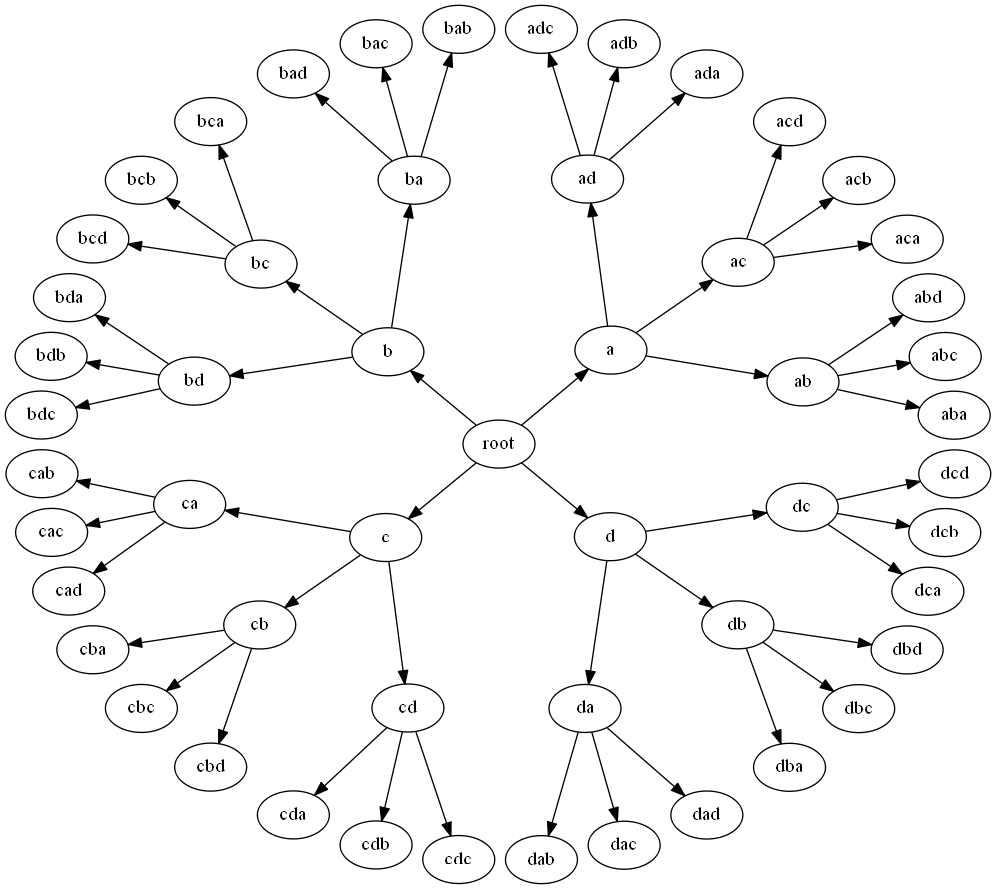
\includegraphics[height=1.35in, keepaspectratio]{img/cayleyGraphabcd.png}
  \caption{\textit{Cayley Graph}}
  \label{fig:cayleyGraph}
  \hspace*{\fill}
 \end{minipage}
 \begin{minipage}[t]{0.5\hsize}
  \center
  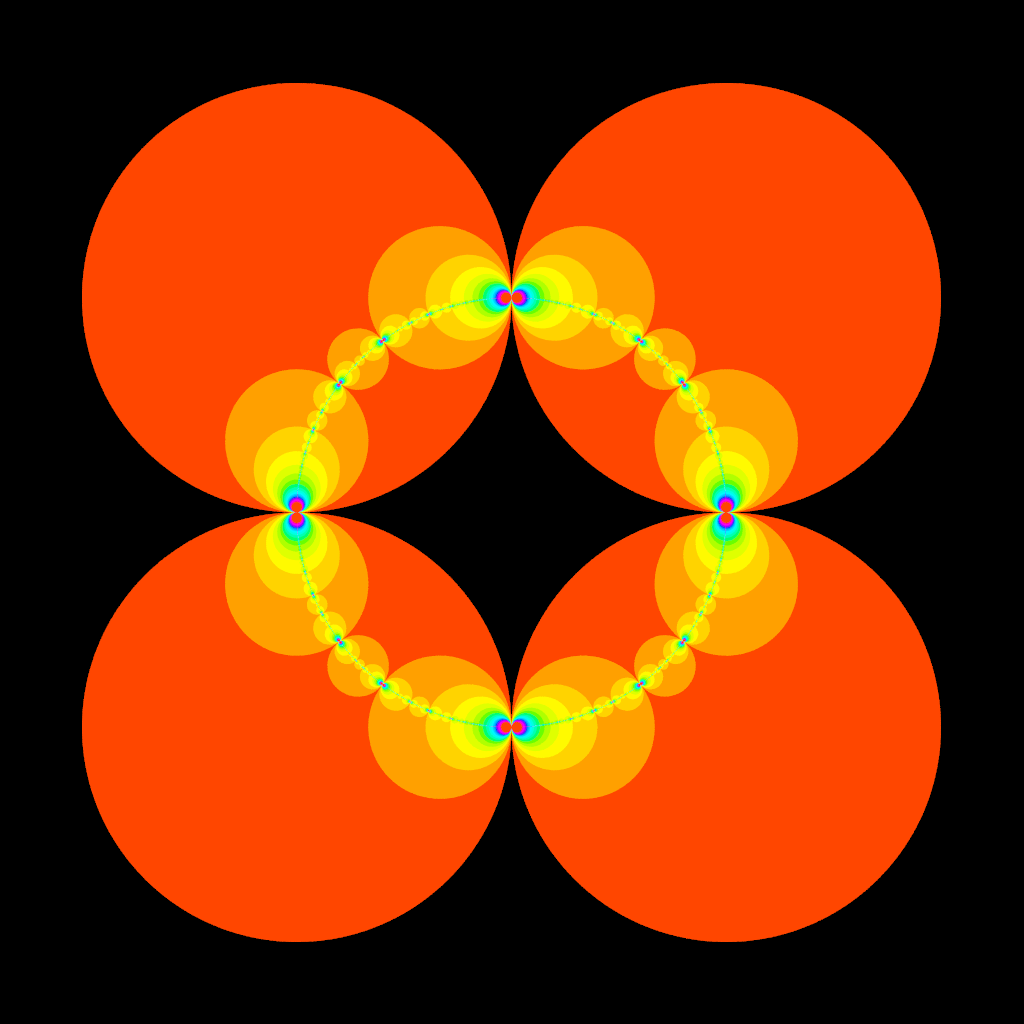
\includegraphics[height=1.35in, keepaspectratio]{img/preparation/basic/circleOrbit.png}
  \caption{\textit{Orbit of the disks}}
  \label{fig:circOrbit}
  \hspace*{\fill}
 \end{minipage}
\end{figure}

\begin{figure}[htbp]
 \begin{minipage}[t]{0.3333\hsize}
  \center
  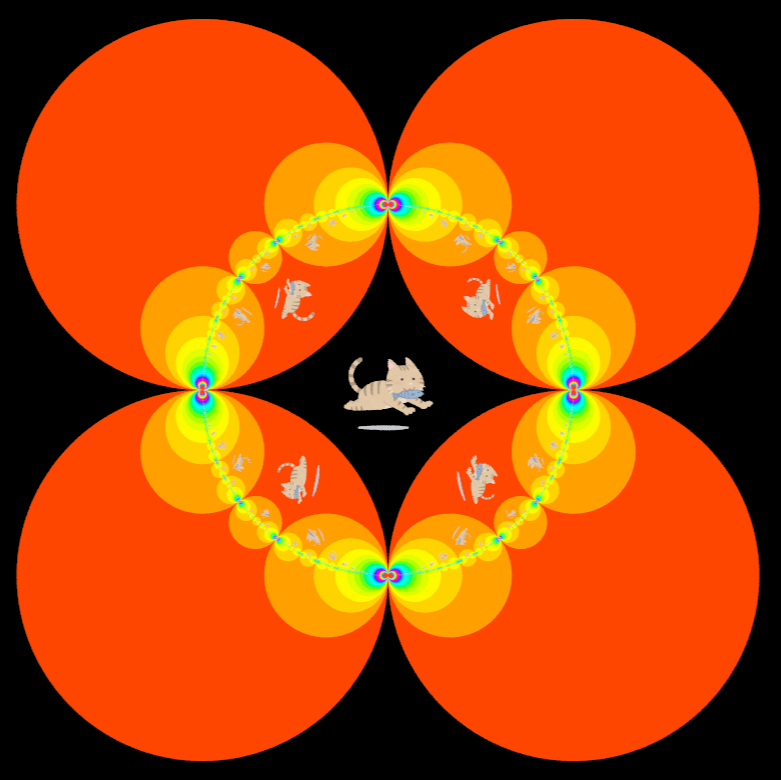
\includegraphics[height=1.35in, keepaspectratio]{img/preparation/basic/catCircleOrbit.png}
  \caption{\textit{The orbit of the cat}}
  \label{fig:orbitCat}
  \hspace*{\fill}
 \end{minipage}
 \begin{minipage}[t]{0.3333\hsize}
  \center
  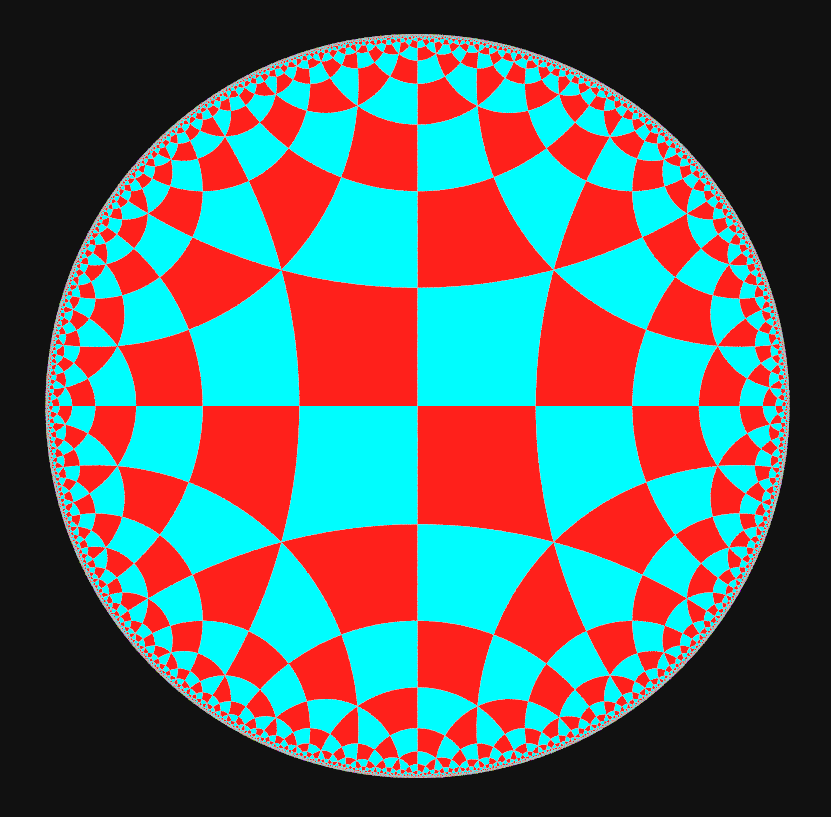
\includegraphics[height=1.35in, keepaspectratio]{img/preparation/basic/hyperbolicTessellation.png}
  \caption{\textit{Hyperbolic Tessellation}}
  \label{fig:hypTiling}
  \hspace*{\fill}
 \end{minipage}
 \begin{minipage}[t]{0.3333\hsize}
  \center
  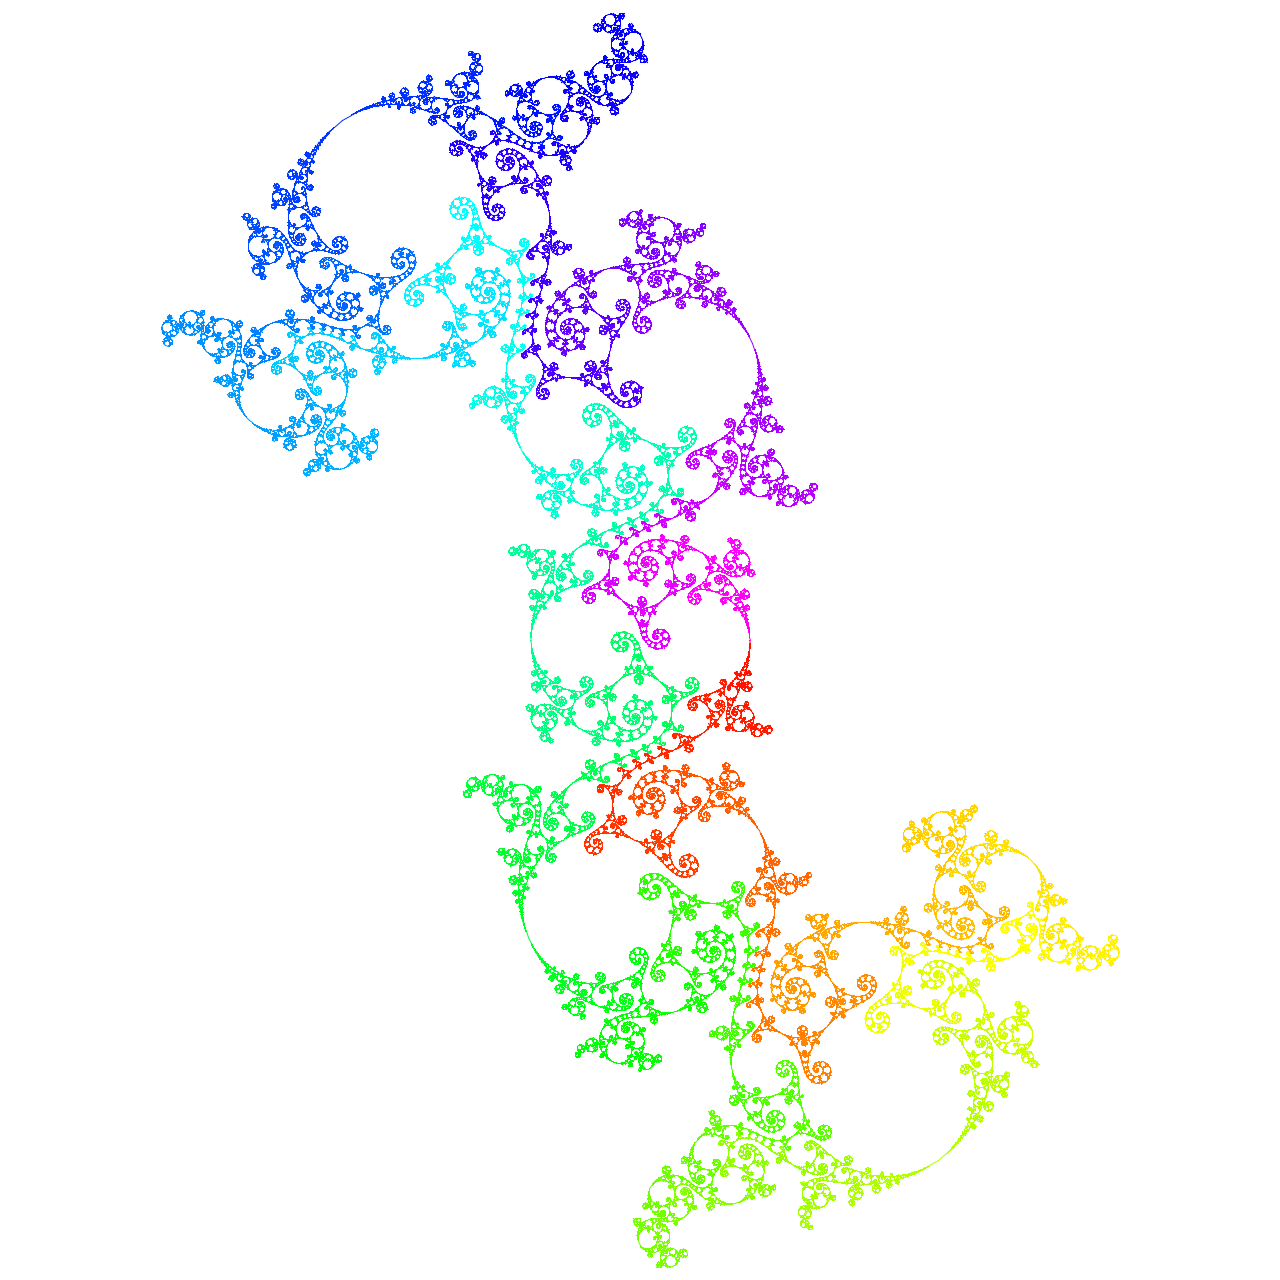
\includegraphics[height=1.35in, keepaspectratio]{img/preparation/limitSet/limit.png}
  \caption{\textit{Limit set of the Kleinian group}}
  \label{fig:limit}
  \hspace*{\fill}
 \end{minipage}
\end{figure}

\noindent In this sub-section, we introduce basic methods for
visualizing extended Kleinian groups.
For simple example, we explain an extended Kleinian group generated by
four inversion mappings.

First of all, to visualize a group we consider \textit{Cayley graph}.
Cayley graph is for a group $G$ given a generators
all elements of $G$ are nodees and multiplication of generators by
right to be related two elements connected by edges.
For an easy example, we assume a group generated by four
involutions, which is a map whose square coincises to the identity.
In short, it is a following group.
\[ G=\langle a,b,c,d \mid a^2=b^2=c^2=d^2 = \mathrm{id} \rangle \]

The Cayley graph of the group is shown in Figure\ref{fig:cayleyGraph}.
The element of the group is nodes. Four edges corresponds to 
$a, b, c, d$ are emitted from each node.
Because $a, b, c, d$ are involution, $a=a^{-1}$ and
an edge corresponds to inverse mapping is not needed.
In Figure \ref{fig:cayleyGraph}, we put identity element $\mathrm{id}$
to center and four edges are stretching symmetrically.
In Cayley graph, length of an edge from identity give the shortest
length of a word.

We can find that the length of the words multiplied by three
that is to say words with length one is four, words with length two are
twelve, words with length three are thirty six, and words with length
$n$ are $4 \cdot 3^{n-1}$

The visualized image is Figure \ref{fig:circOrbit}. In this image,
we draw four circles on the plane, and we call their inversion mapping
$a, b, c,$ and $ d$ respectively. Four circles come in touch, but do not cross,
and there are no relational expression between $a$, $b$, $c$, and $d$.
Thus, extended M\"obius transformation group generated by four inversion
mapping is isomorphic group to $G$ above.
In Figure \ref{fig:orbitCat}, the cat drew in center are moved by
inversion mapping, and visualized ``orbit space of the cat''.
We can find that the orbit space of the cat corresponds to nodes of
the graph.

In order to draw orbit space of the cat, there are breadth first search
algorithm.
In the following, we explain breadth first search algorithm.
First of all, we draw the cat in center, and
Next, we draw transformed cat by the words whose length is one,
and we draw transformed cat by the word whose length is two.
We continue iterating these processes.
This is breadth first search algorithm.
The tessellation shown in Figure \ref{fig:hypTiling} is also drawn by
Breadth First Search Algorithm.

Visualization of this algorithm are easy to implement and understand.
We can roughly understand its actions of the groups.
However, there are defective what the computational complexity is 
easy to increase and it takes too much times.

Also, there is one more method of traversing graph.
It is called depth first search.
This one can draw only limit set directly.
See Figure \ref{fig:limit}. This shows an only limit set of a Kleinian
group.
However, we do not use this algorithm in this paper.
For more details of the algorithm, read \cite{MumfordSeriesWright200204}.

\subsection{Iterated Inversion System (IIS)}

\begin{figure}[htbp]
 \begin{minipage}[t]{0.16\hsize}
  \center
  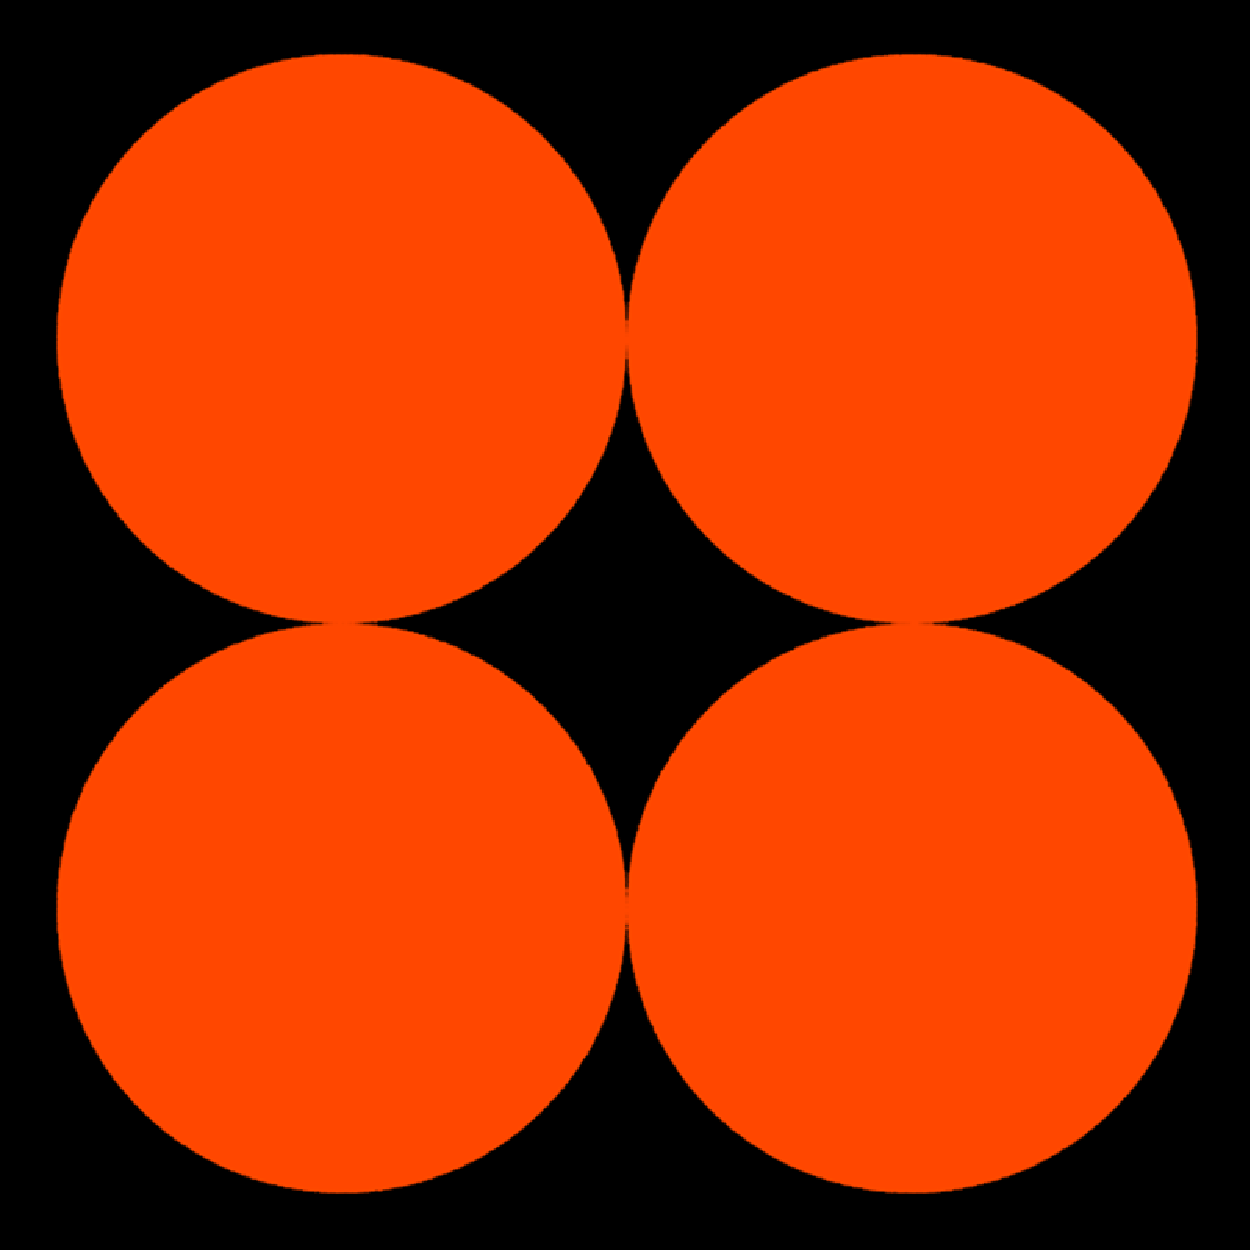
\includegraphics[width=1in, height=1in, keepaspectratio]{./img/preparation/orbit/level0c.pdf}
  \subcaption{}
  \label{fig:level0}
 \end{minipage}
 \begin{minipage}[t]{0.16\hsize}
  \center
  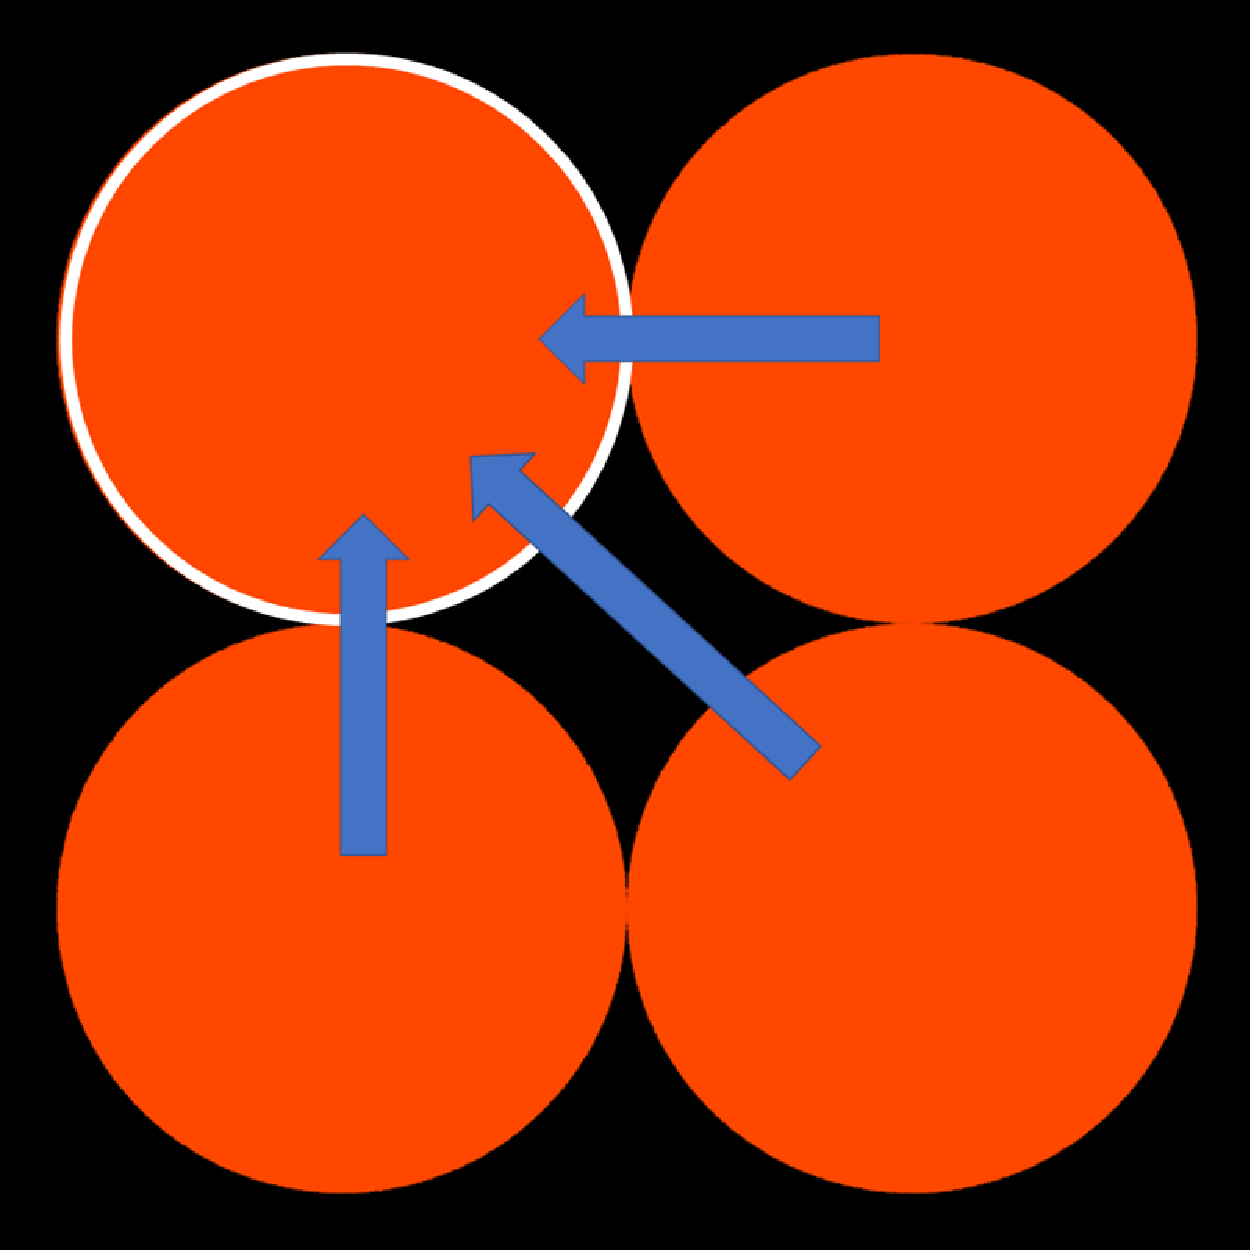
\includegraphics[width=1in, height=1in, keepaspectratio]{./img/preparation/orbit/level0invc.pdf}
  \subcaption{}
   \label{fig:level0inv}
 \end{minipage}
 \begin{minipage}[t]{0.16\hsize}
  \center
  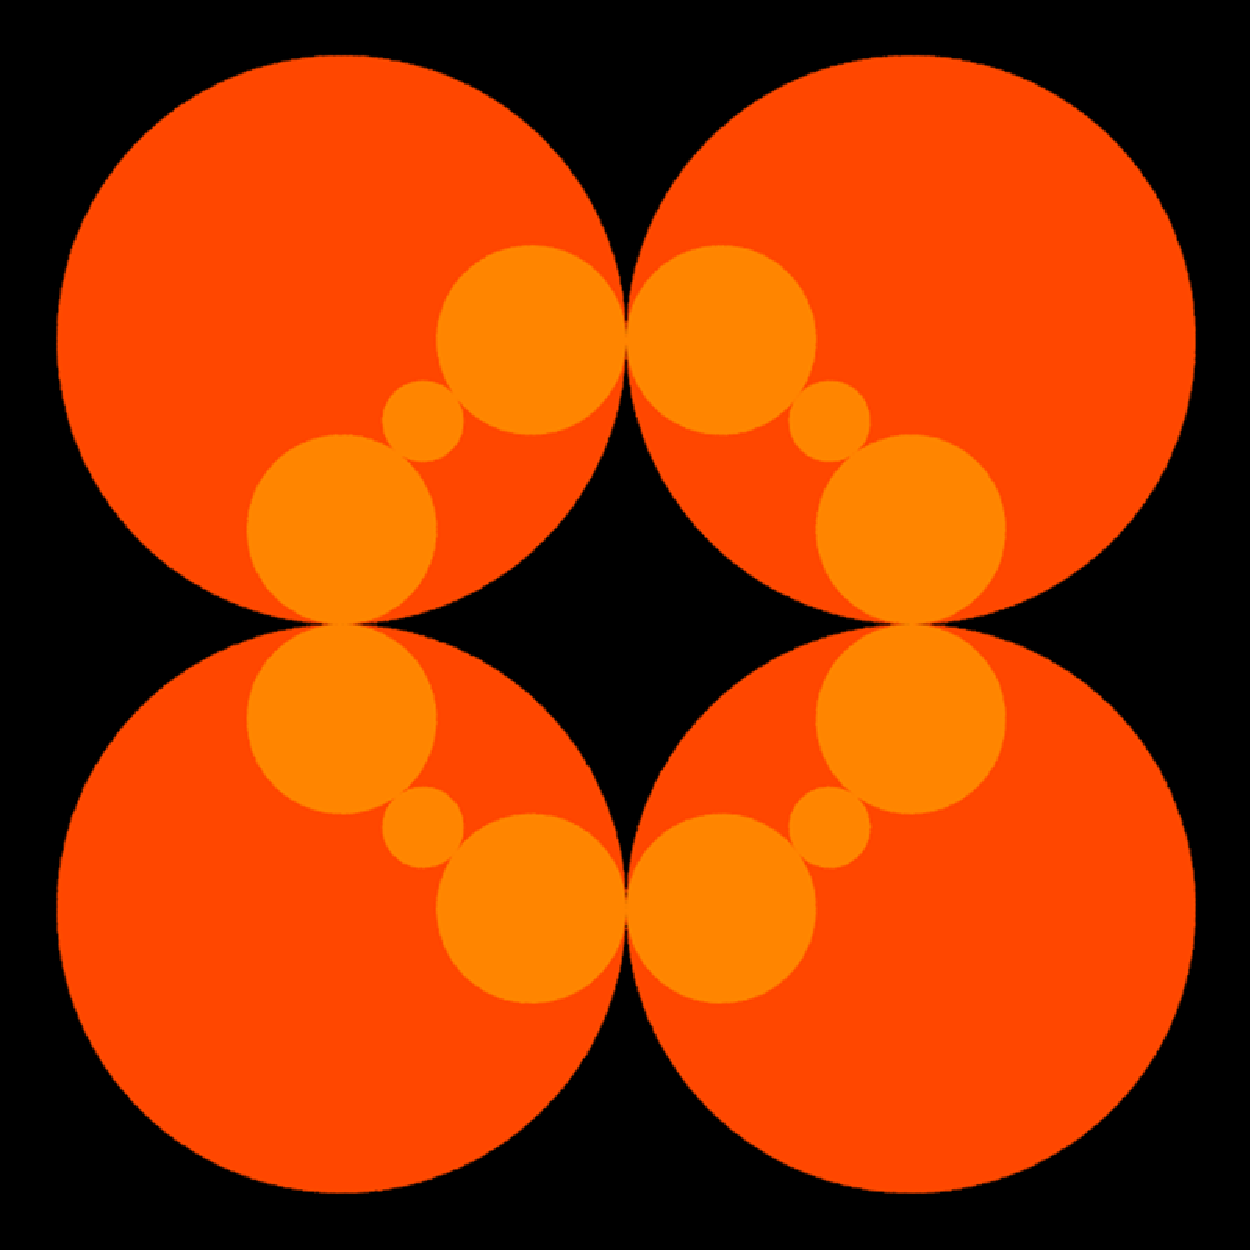
\includegraphics[width=1in, height=1in, keepaspectratio]{./img/preparation/orbit/level1c.pdf}
  \subcaption{}
   \label{fig:level1}
 \end{minipage}
 \begin{minipage}[t]{0.16\hsize}
  \center
  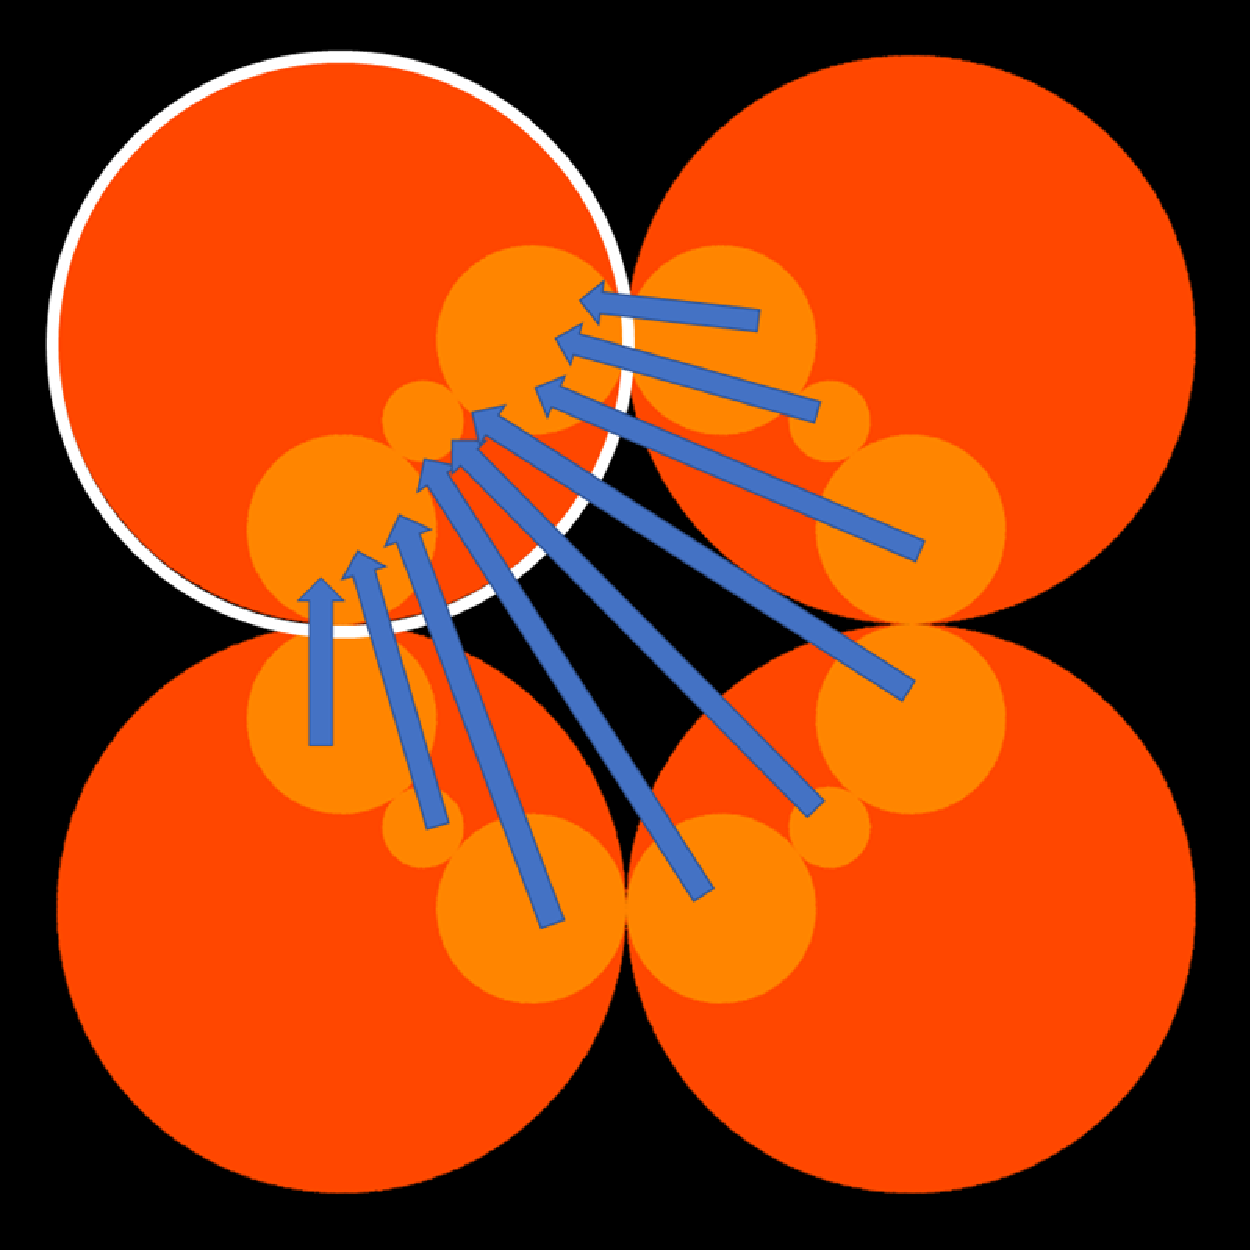
\includegraphics[width=1in, height=1in,
  keepaspectratio]{./img/preparation/orbit/level1invc.pdf}
  \subcaption{}
  \label{fig:level1inv}
 \end{minipage}
 \begin{minipage}[t]{0.16\hsize}
  \center
  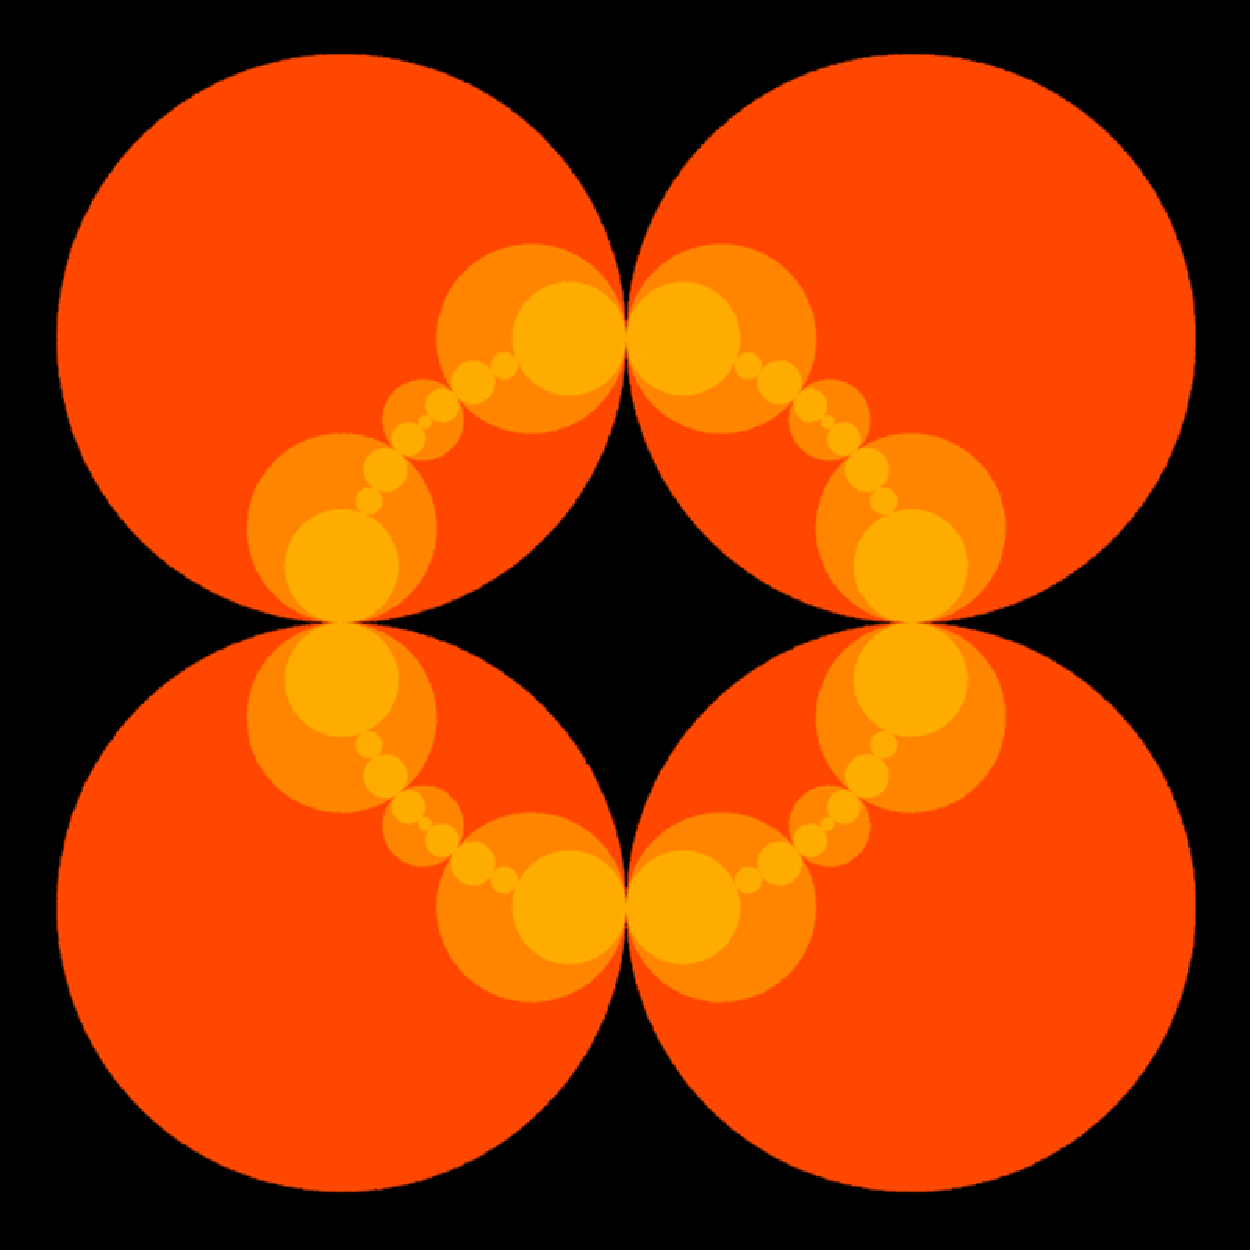
\includegraphics[width=1in, height=1in, keepaspectratio]{./img/preparation/orbit/level2c.pdf}
  \subcaption{}
  \label{fig:level2}
 \end{minipage}
 \begin{minipage}[t]{0.16\hsize}
  \center
  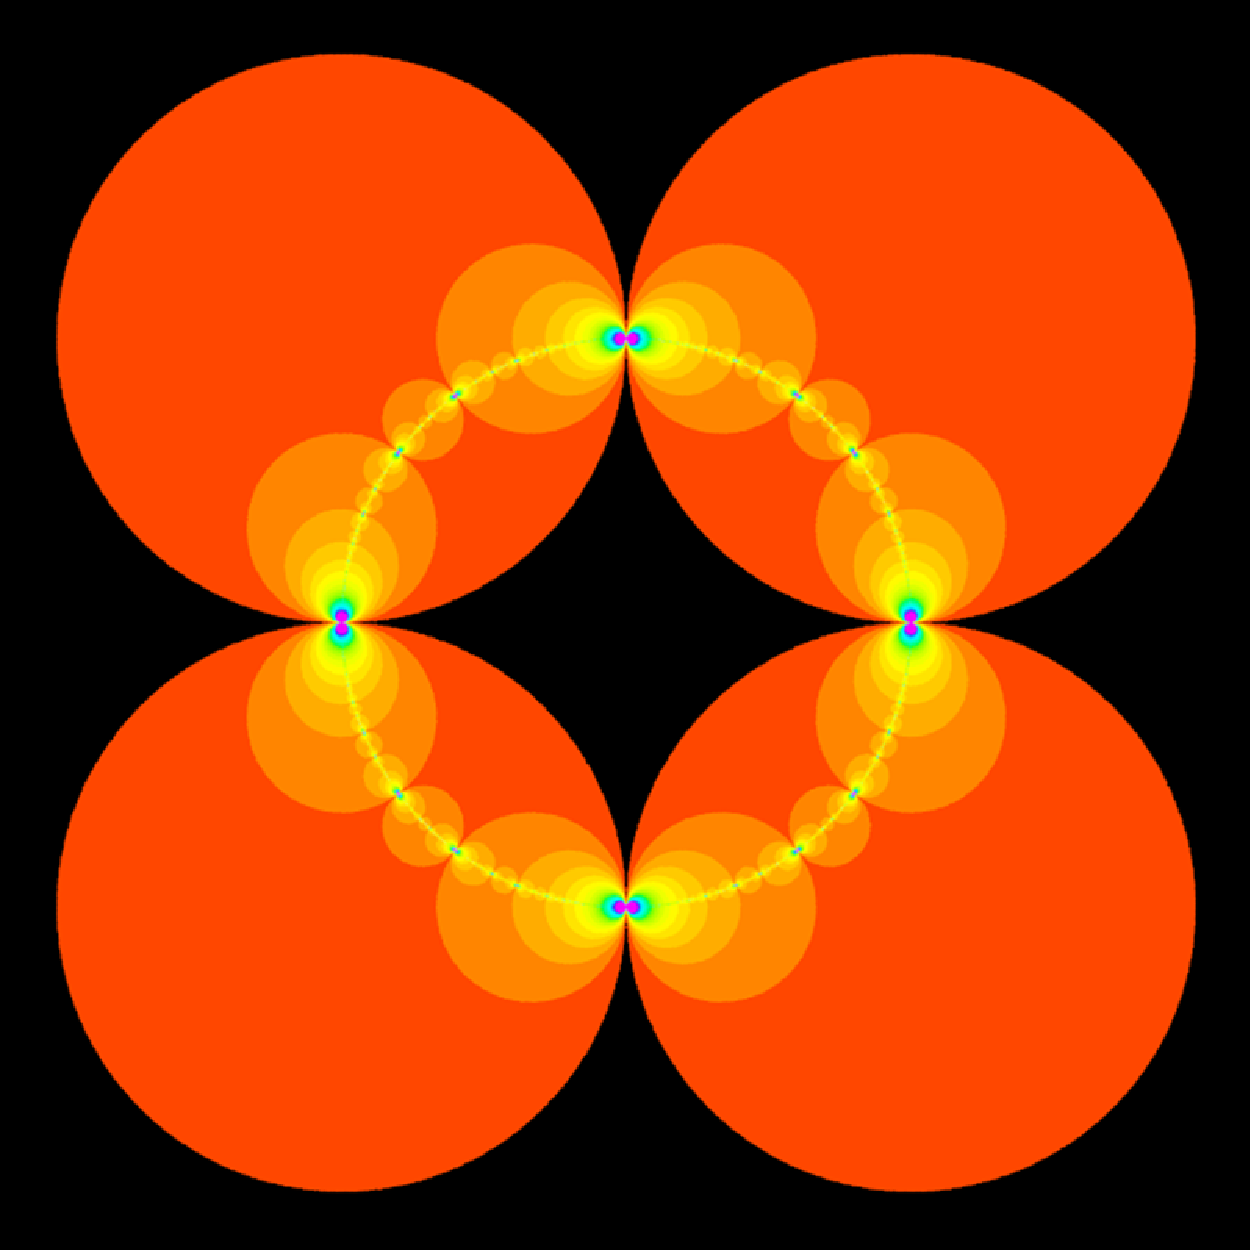
\includegraphics[width=1in, height=1in, keepaspectratio]{img/preparation/orbit/levelMaxc.pdf}
  \subcaption{}
  \label{fig:levelMax}
 \end{minipage}
 \caption{\textit{The process of rendering the orbit of Schottky disks}}
 \label{fig:schottkyProcess}
\end{figure}

\noindent To solve the problems we discussed in the previous sub-section,
we focus circle inversions and invent an efficient algorithm to
visualize circle inversion fractals shown in Figure \ref{fig:schottkyProcess}\subref{fig:levelMax}.
The algorithm is called \textit{Iterated Inversion System (IIS.)}
It can visualize not only two-dimensional circle inversion fractals but
also three-dimensional sphere inversion fractals.

The fractal in Figure \ref{fig:schottkyProcess}\subref{fig:levelMax} shows the orbit of the first
four circles in Figure \ref{fig:schottkyProcess}\subref{fig:level0}. %% TODO もうすこし説明を加える
It is also a Kleinian group composed of four circle inversions.
Especially, it is called a \textit{quasi-fuchsian group}.
The process of generation of circle inversion fractals is
as follows.

\begin{enumerate}
 \item We need some disjoint disks to obtain circle inversion fractals.
       For example, we assume there are four orange disks as shown in
       Figure \ref{fig:schottkyProcess}\subref{fig:level0}. We call orange disks \textit{initial
       disks} and their boundary \textit{initial circles}.
 \item First of all, we focus on the white circle in Figure
       \ref{fig:schottkyProcess}\subref{fig:level0inv}. The inversion in the white circle moves the
       other three disks into the interior of the white circle.
 \item After we apply each inversion in the initial circle to the outer disks,
       we obtain twelve small disks. They are shown in Figure \ref{fig:schottkyProcess}\subref{fig:level1}.
 \item Next, we invert the twelve small disks in the initial circles.
       The inversion in the white circle moves the outer nine small disks
       into the interior of the white circle as shown in Figure \ref{fig:schottkyProcess}\subref{fig:level1inv}.
       Each inversion in the Schottky circle generates smaller disks, and we
       obtain Figure \ref{fig:schottkyProcess}\subref{fig:level2}.
 \item We continue iterating these process, that is, we continue
       applying each inversion in the initial circle to resulting
       smaller disks.
       Finally, we get Figure \ref{fig:schottkyProcess}\subref{fig:levelMax}.
\end{enumerate}

\subsubsection{Two Dimensional IIS}

\begin{figure}[htbp]
  \center
  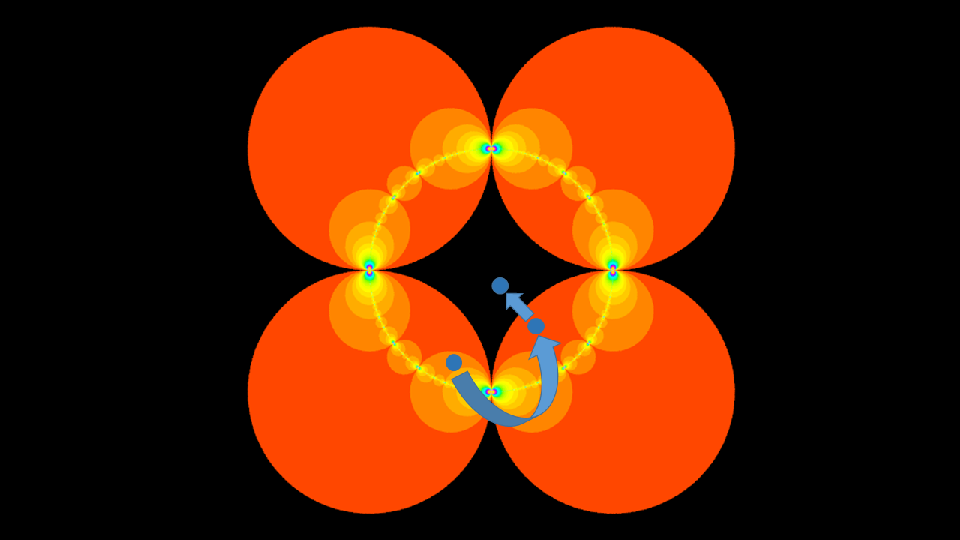
\includegraphics[height=1.35in, keepaspectratio]{img/preparation/orbIIS.png}
  \caption{\textit{Orbit of blue point by IIS}}
  \label{fig:iisOrbit}
 \hspace*{\fill}
\end{figure}

 \begin{algorithm}
  \caption{Iterated Inversion System (IIS)}
  \label{arg:iis2d}
  \begin{algorithmic}
   \REQUIRE count $= 0$ and coordinates $=$ position determined by
   pixel
   \FOR{$i=0$ to MAX\_INVERSION}
   \STATE inOutside $\leftarrow$ \TRUE
   \FOR{ each Map $G$ in circles }
   \IF{$G$ is available to coordinates}
   \STATE coordinates $\leftarrow$ $G(\text{coordinates})$
   \STATE INCREMENT count
   \STATE inOutside $\leftarrow$ \FALSE
   \ENDIF
   \ENDFOR
   \IF {inOutside}
   \STATE BREAK for
   \ENDIF
   \ENDFOR
   \STATE RETURN count
  \end{algorithmic}
 \end{algorithm}

\noindent IIS computes the depth of the circles point by point.
Thus, we can perform parallel processing and render the images efficiently.
The images in this paper are rendered using \textit{OpenGL Shading
Language (GLSL)}.

IIS is applied to each point on the plane and computes nesting depth of
the disk which contains the point.
The process of the algorithm is as follows.
First of all, if the point is contained in initial disks, we invert the
point in the boundary circle of the disk.
We continue applying inversions until the transformed point is in the
outside of the initial disks.
Figure \ref{fig:iisOrbit} shows the orbit of the blue point transformed by
iterations of inversions.

Furthermore, a point actually at the limit set never reaches the
outside. So, we have to determine the maximum number of iterations in
advance to prevent the algorithm from running indefinitely.
The points except for the limit set are guaranteed that they
are transformed to outside because inversions are involution.

Pseudo-code of IIS is shown in Algorithm \ref{arg:iis2d}.
Later, we will introduce generators other than simple inversions.
Thus, we consider a map $G$ such that $G$ is an identity for a point in the
\textit{fundamental domain} and that $G$ is a composition of inversions for other
points.
The fundamental domain is the terminal area of transformations. 
In the above case, the black area where outside of all circles.

\subsubsection{Three Dimensional Extension}

\begin{figure}[htbp]
 \begin{minipage}[t]{0.5\hsize}
  \center
  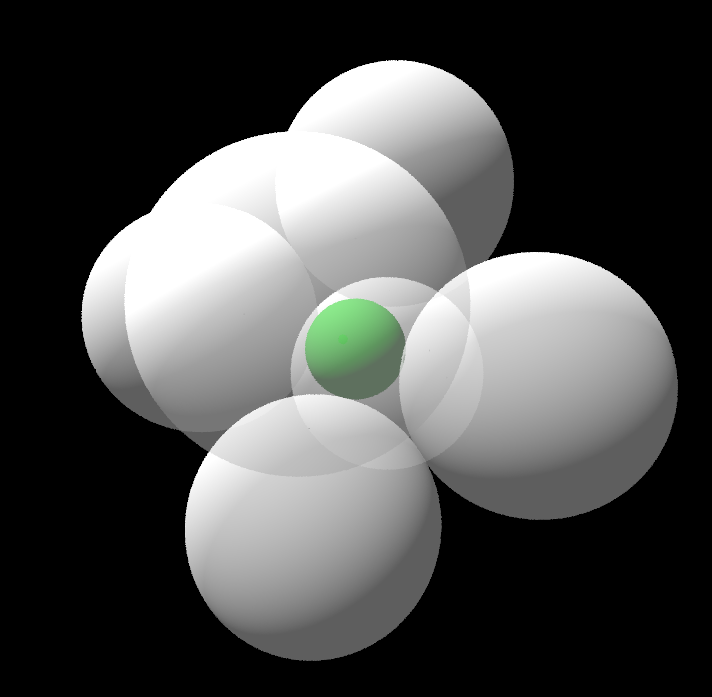
\includegraphics[height=1.35in, keepaspectratio]{img/preparation/3dExtension/3dKissingGenerator.png}
  \subcaption{\textit{Generator}}
  \label{fig:simpleGen}
  \hspace*{\fill}
 \end{minipage}
 \begin{minipage}[t]{0.5\hsize}
  \center
  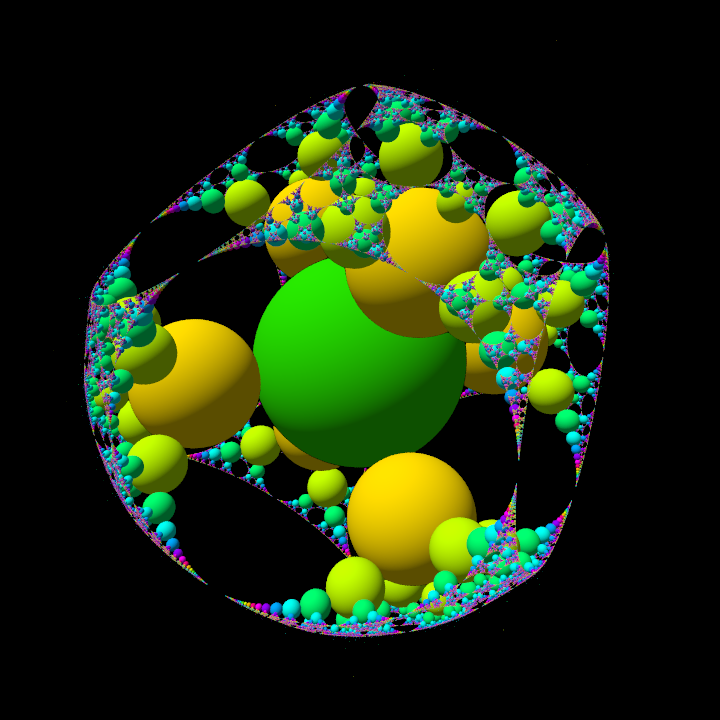
\includegraphics[height=1.35in, keepaspectratio]{img/preparation/3dExtension/3dOrbit.png}
  \subcaption{\textit{The orbit of spheres}}
  \label{fig:simpleOrb}
  \hspace*{\fill}
 \end{minipage}
 \caption{\textit{The orbit of the sphere inversion fractal}}
 \label{fig:simpleGenOrb}
\end{figure}

\begin{figure}[htbp]
 \begin{minipage}[t]{0.5\hsize}
  \center
  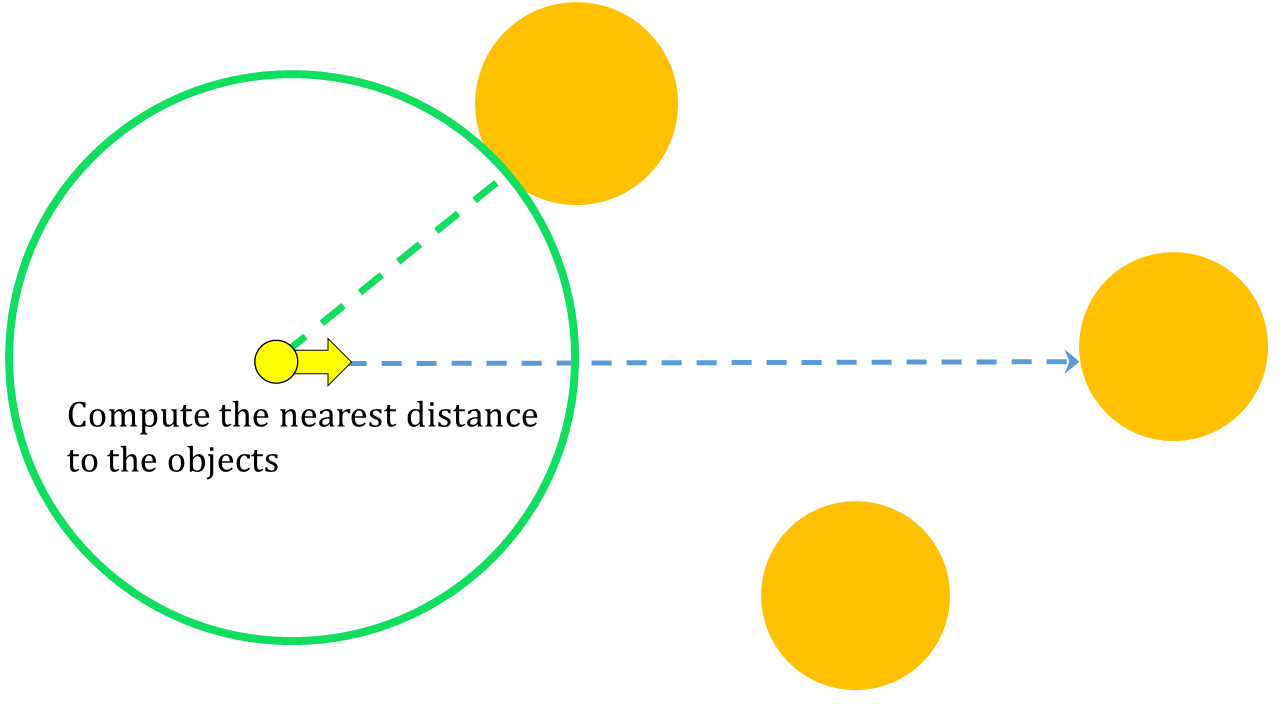
\includegraphics[height=1.35in, keepaspectratio]{img/visualization/sphereTracing1.png}
  \subcaption{\textit{}}
  \label{fig:st1}
  \hspace*{\fill}
 \end{minipage}
 \begin{minipage}[t]{0.5\hsize}
  \center
  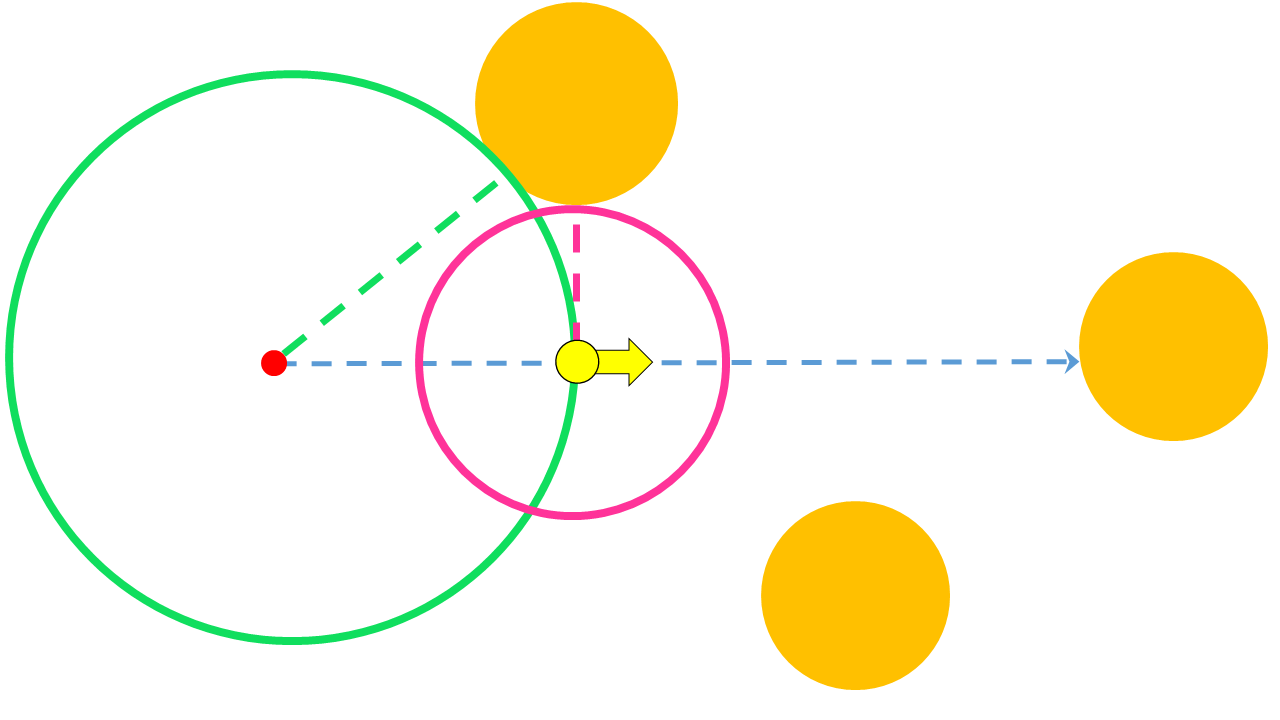
\includegraphics[height=1.35in, keepaspectratio]{img/visualization/sphereTracing2.png}
  \subcaption{\textit{}}
  \label{fig:st2}
  \hspace*{\fill}
 \end{minipage}
 \begin{minipage}[t]{0.5\hsize}
  \center
  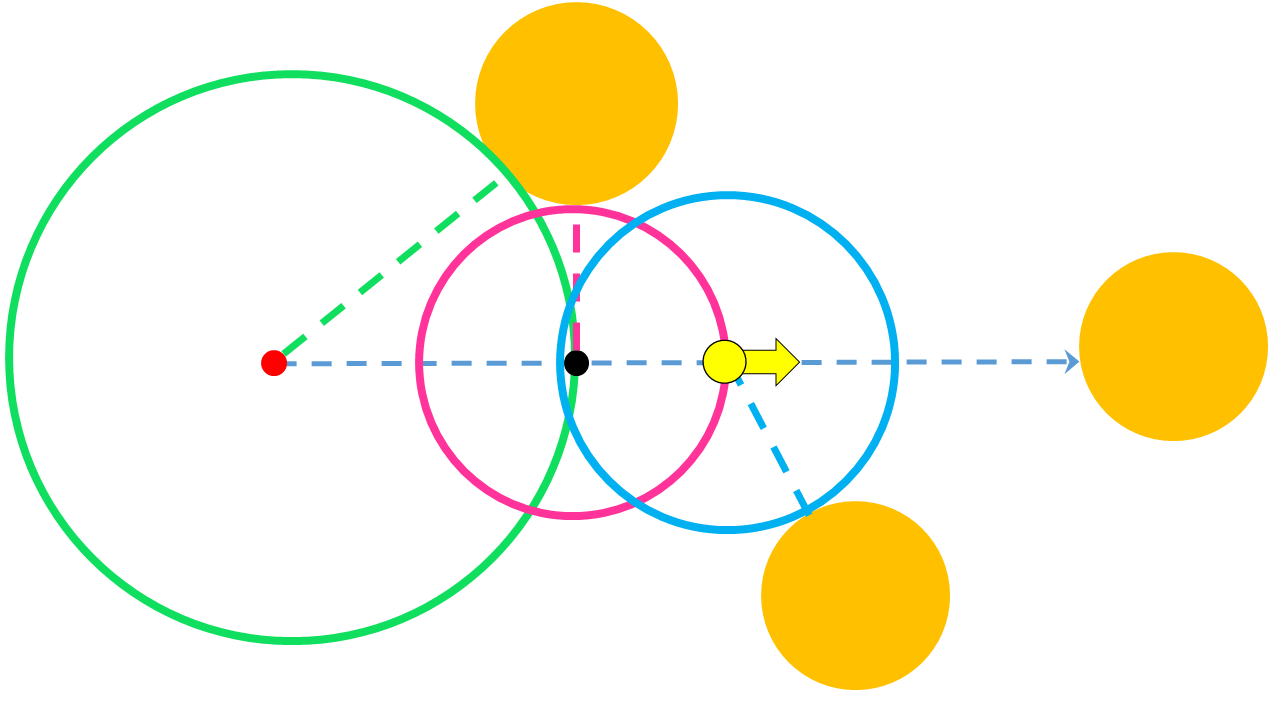
\includegraphics[height=1.35in, keepaspectratio]{img/visualization/sphereTracing3.png}
  \subcaption{\textit{}}
  \label{fig:st3}
  \hspace*{\fill}
 \end{minipage}
 \begin{minipage}[t]{0.5\hsize}
  \center
  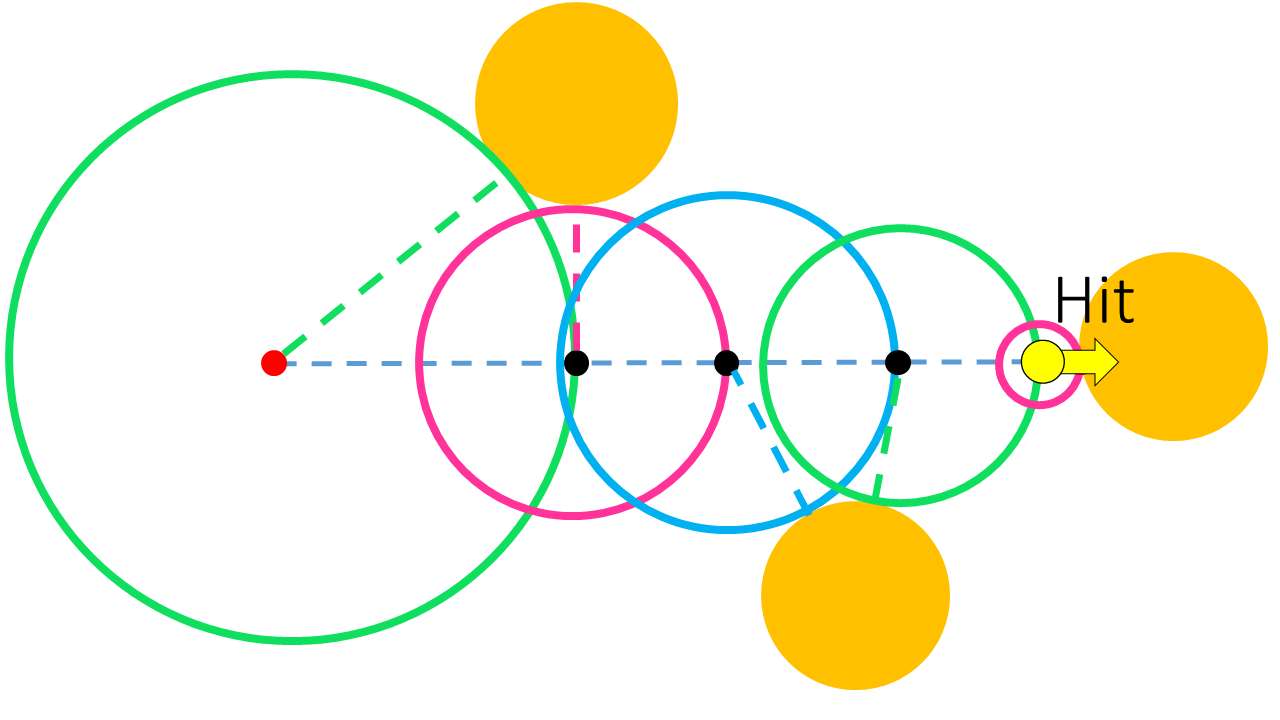
\includegraphics[height=1.35in, keepaspectratio]{img/visualization/sphereTracing4.png}
  \subcaption{\textit{}}
  \label{fig:st4}
  \hspace*{\fill}
 \end{minipage}
 \caption{\textit{Sphere tracing}}
 \label{fig:sphereTracing}
\end{figure}

In a similar manner to the two-dimensional algorithm,
we extend the IIS to visualize three-dimensional Kleinian groups.
We extend circle inversion to sphere inversion easily, and we
compute the nesting depth of the sphere voxel by voxel.

We use \textit{ray tracing} to visualize three-dimensional objects.
Ray tracing computes an intersection between a ray and objects
algebraically.
There are two ways to render nesting spheres. First one is to draw
nesting spheres as transparent spheres.
Second one is \textit{volume rendering}.
However, these are difficult to render them efficiently, and
visualized images are not interesting.

Therefore we render the orbit of the sphere in a similar way to the
two-dimensional circle inversion fractals.
See Figure \ref{fig:simpleGenOrb}\subref{fig:simpleGen}. It shows
white six inversion spheres and a green seed sphere.
Figure \ref{fig:simpleGenOrb}\subref{fig:simpleOrb} shows the orbit of
the green sphere transformed by inversions in white spheres.

We use \textit{Sphere Tracing} \cite{hart1996sphere} to render three-dimensional
fractals and orbit of the seed sphere.
Sphere Tracing is one of the algorithms to render implicit surfaces using
ray tracing.
In the following paragraphs, we introduce ray tracing and
sphere tracing.

In the first place, we work a ray as something like a vector.
We set the origin of the ray to the position of the camera
and direction of the ray to the direction to each pixel on the screen
from the camera. Each pixel is colored according to the
first object the ray hits. 

In regular ray tracing, we calculate the intersections algebraically, but
we can not compute intersection to fractal objects.
On the other hand, in sphere tracing, we march the ``tip'' of the ray
along the direction of the ray step by step. 
To check how far the tip of the ray is from the objects, we need a
\textit{distance function}.
The distance function is a function which returns the minimum distance
between given point and objects.
For example, a distance function of a sphere is as follows.
Let $P$ be a tip of a ray, let $C$ and $R$ be center and
radius of the sphere.
Distance function $f(P)$ is $f(P) = distance(P, C) - R$.
If there are many spheres, we use minimum distance to the sphere.

Figure \ref{fig:sphereTracing} shows sphere tracing algorithm.
The yellow arrow is ray and orange disks are visible objects.
First of all, in Figure Figure \ref{fig:sphereTracing}\subref{fig:st1},
we use distance function and find minimum distance between
the ray and the disk.
Next, we put the ray forward and apply distance function to the position
of the ray as in Figure \ref{fig:sphereTracing}\subref{fig:st2}.
Again, we apply distance function and march the ray, and we obtain
Figure \ref{fig:sphereTracing}\subref{fig:st3}.
We continue iterating this processes until the value of the distance
function is less than zero as shown in Figure \ref{fig:sphereTracing}\subref{fig:st4}.

However, in regard to fractal rendering, it is difficult to
get an actual distance to its shape. So, we use a lower estimated distance
as a return value of the distance function. The technique to approximate
distance is called \textit{distance estimation}.
For more details about fractal rendering and distance estimation, see also the blog
post\footnote{Mikael H Christensen, Distance Estimated 3D Fractals (Part I):\\ \quad\quad
\url{http://blog.hvidtfeldts.net/index.php/2011/06/distance-estimated-3d-fractals-part-i/}}
by Christensen. 

\begin{figure}[htbp]
 \begin{minipage}[t]{0.5\hsize}
  \center
  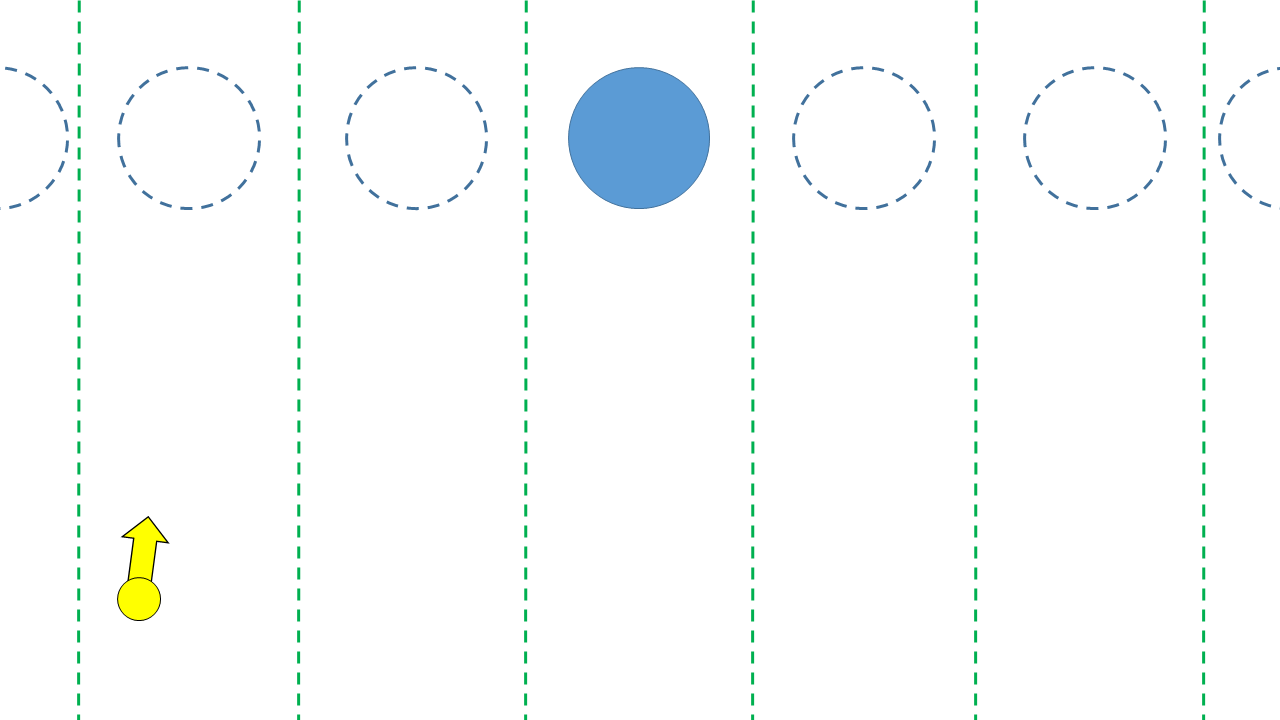
\includegraphics[height=1.35in, keepaspectratio]{img/visualization/translate1.png}
  \subcaption{\textit{}}
  \label{fig:modulo1}
  \hspace*{\fill}
 \end{minipage}
 \begin{minipage}[t]{0.5\hsize}
  \center
  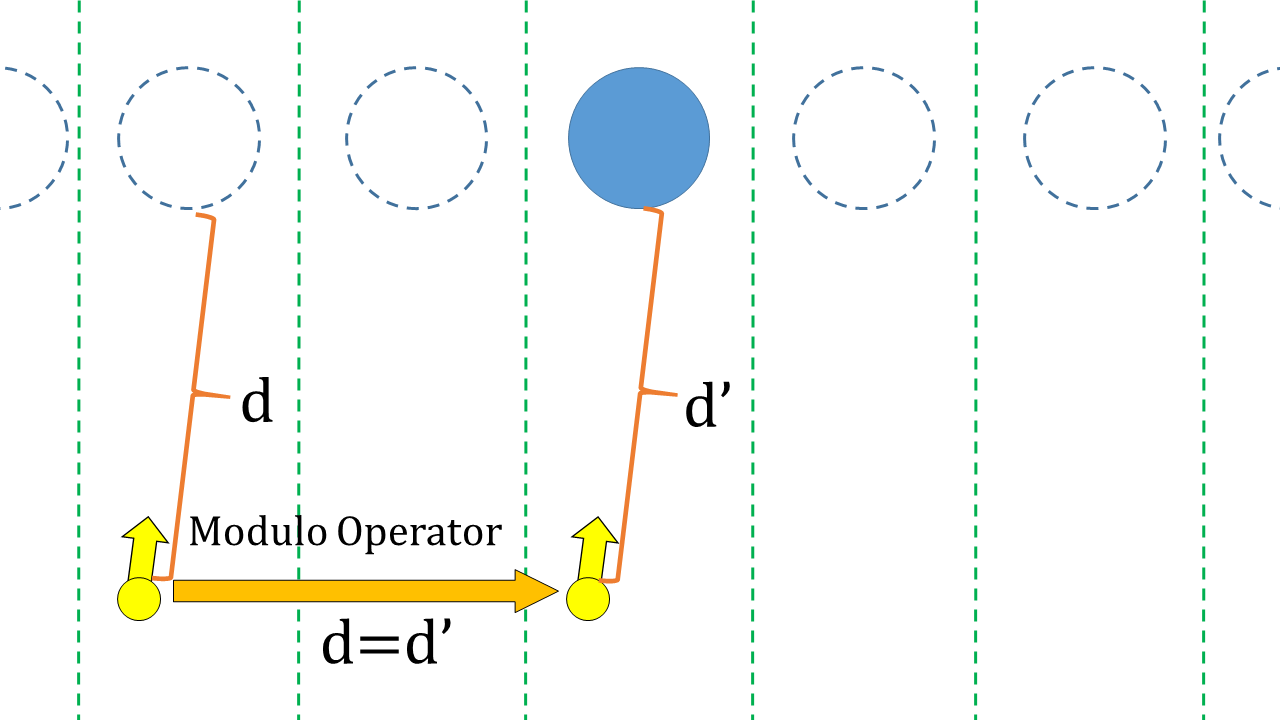
\includegraphics[height=1.35in, keepaspectratio]{img/visualization/translate2.png}
  \subcaption{\textit{}}
  \label{fig:modulo2}
  \hspace*{\fill}
 \end{minipage}
 \caption{\textit{Fold space by modulo operator}}
 \label{fig:moduloAll}
\end{figure}

\begin{figure}[htbp]
 \begin{minipage}[t]{0.5\hsize}
  \center
  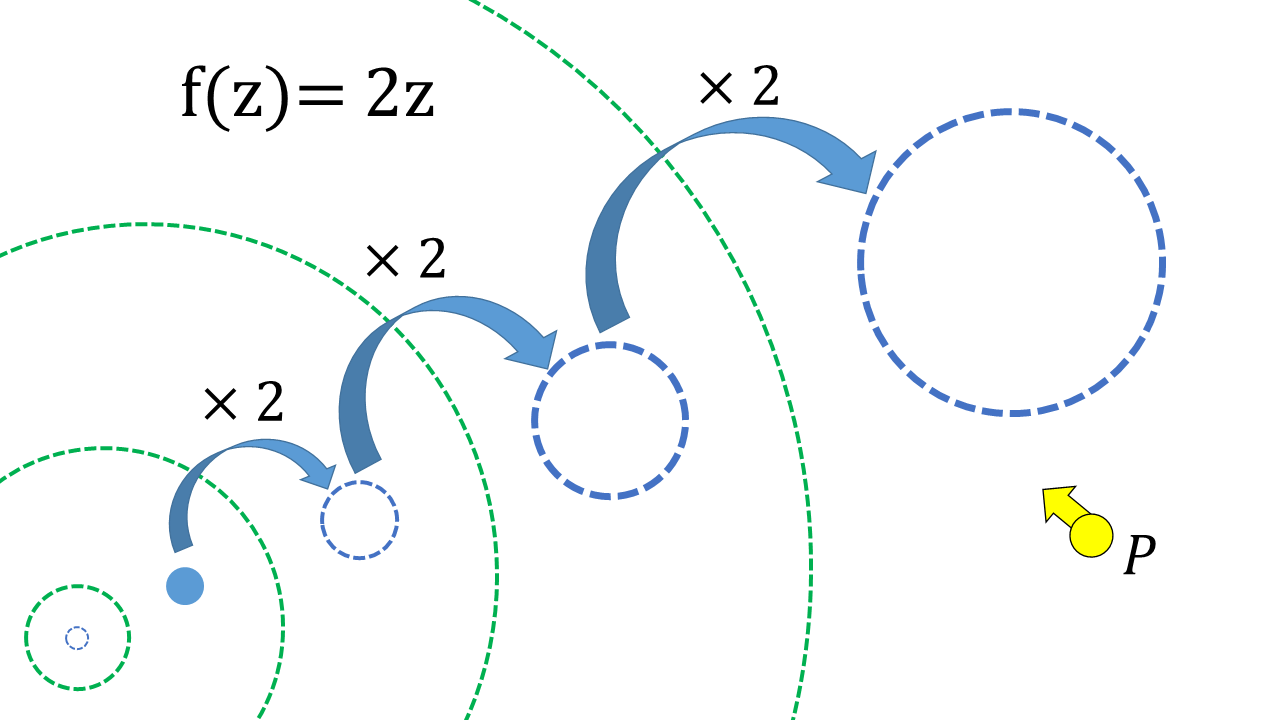
\includegraphics[height=1.35in, keepaspectratio]{img/visualization/scaling1.png}
  \subcaption{\textit{}}
  \label{fig:iisScale1}
  \hspace*{\fill}
 \end{minipage}
 \begin{minipage}[t]{0.5\hsize}
  \center
  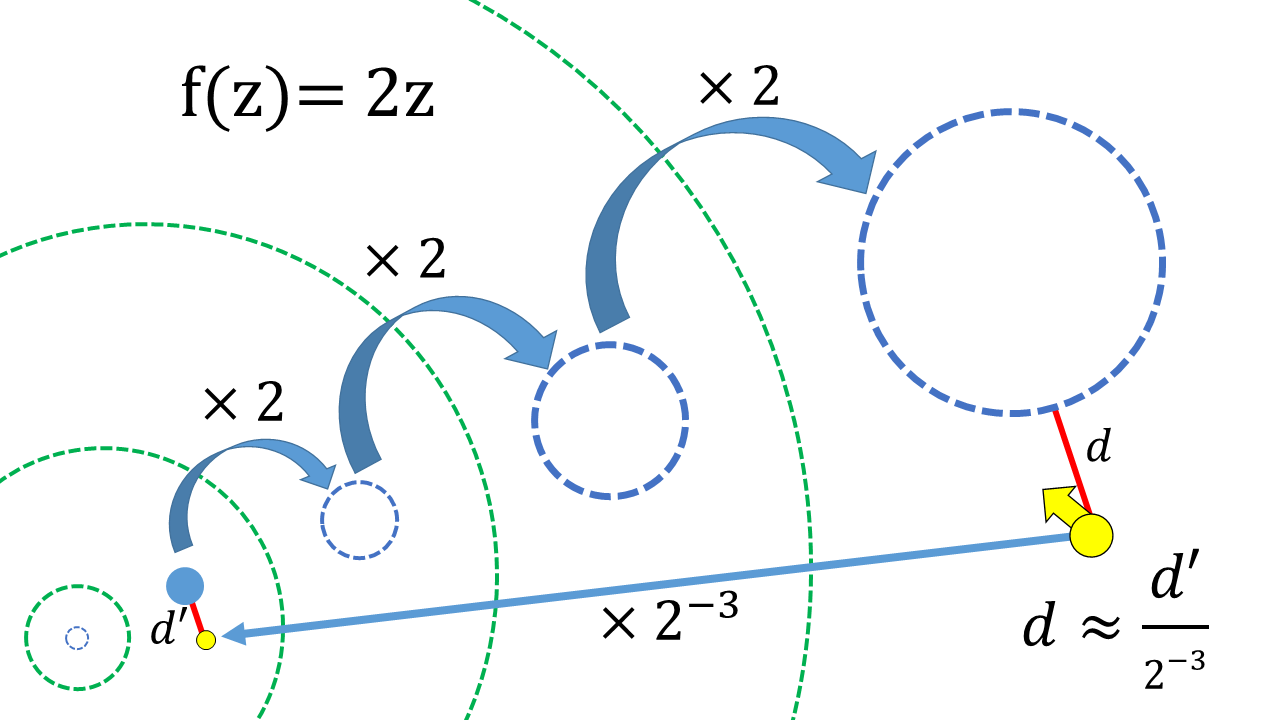
\includegraphics[height=1.35in, keepaspectratio]{img/visualization/scaling2.png}
  \subcaption{\textit{}}
  \label{fig:iisScale2}
  \hspace*{\fill}
 \end{minipage}
 \caption{\textit{Fold space by scaling}}
 \label{fig:iisScaleAll}
\end{figure}

Before we introduce distance estimation, we show
well-known technique to render many objects in sphere tracing.
Instead of preparing distance functions for many objects, we can use modulo operator
to get the distance to the lined up objects.

See Figure \ref{fig:moduloAll}\subref{fig:modulo1}. We assume there are the blue disk, the
yellow ray, and dotted circle and lines.
Now, we want to draw all of the dotted circles.
So, we want a minimum distance between the ray and dotted circles.
However, we only know the position of the tip of the ray and the blue disk.
Thus, we assume the nearest circle to the ray is in the same dotted region, and
we fold up the regions using the modulo operator.
We can measure the distance to blue disk as in Figure \ref{fig:moduloAll}\subref{fig:modulo2}.
Finally, we can draw line upped disks.

Next, we consider scaling example.
See Figure \ref{fig:iisScaleAll}\subref{fig:iisScale1}.
There are a yellow ray and a blue disk, and orbit of scaling as
dotted blue circles.
The green dotted lines show scaling regions.
We want to minimum distance between dotted blue circles and the ray.
However, we only know the coordinates of the original blue
disk and tip of the ray.
We assume that the nearest sphere to the tip of the ray is in
same regions. 
Thus, we scale the tip of the ray to the same region to the blue disk
but, the distance between scaled ray and disk is also scaled.
So, we correct the scale dividing computed distance by 
Jacobian (sometimes referred to as the Jacobian determinant) of scaling.
See Figure \ref{fig:iisScaleAll}\subref{fig:iisScale2}.
If the scaling of the circle is $f(x) = 2x$, we divide the scale by
eight because the ray is moved three green scaling regions.

\begin{figure}[htbp]
 \begin{minipage}[t]{0.5\hsize}
  \center
  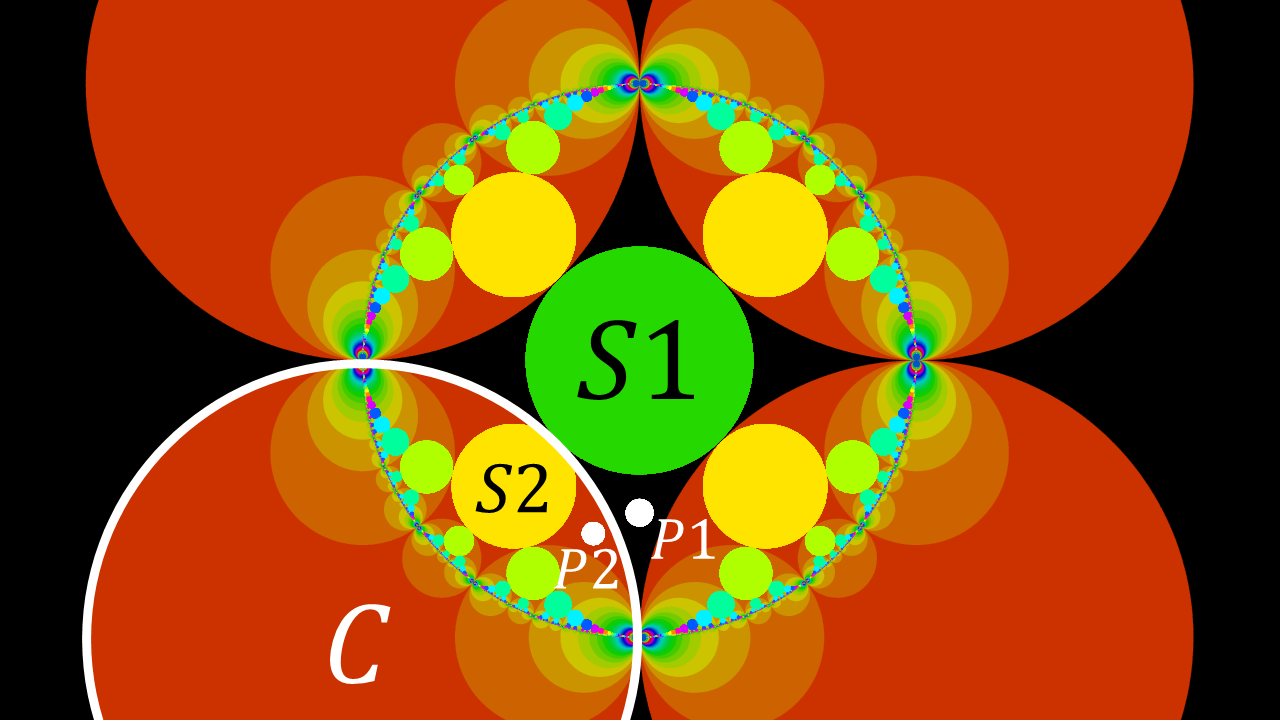
\includegraphics[height=1.35in, keepaspectratio]{img/preparation/slice.png}
  \caption{\textit{XY-slice image of Figure \ref{fig:simpleGenOrb}\subref{fig:simpleOrb}}}
  \label{fig:slice2d}
  \hspace*{\fill}
 \end{minipage}
 \begin{minipage}[t]{0.5\hsize}
  \center
  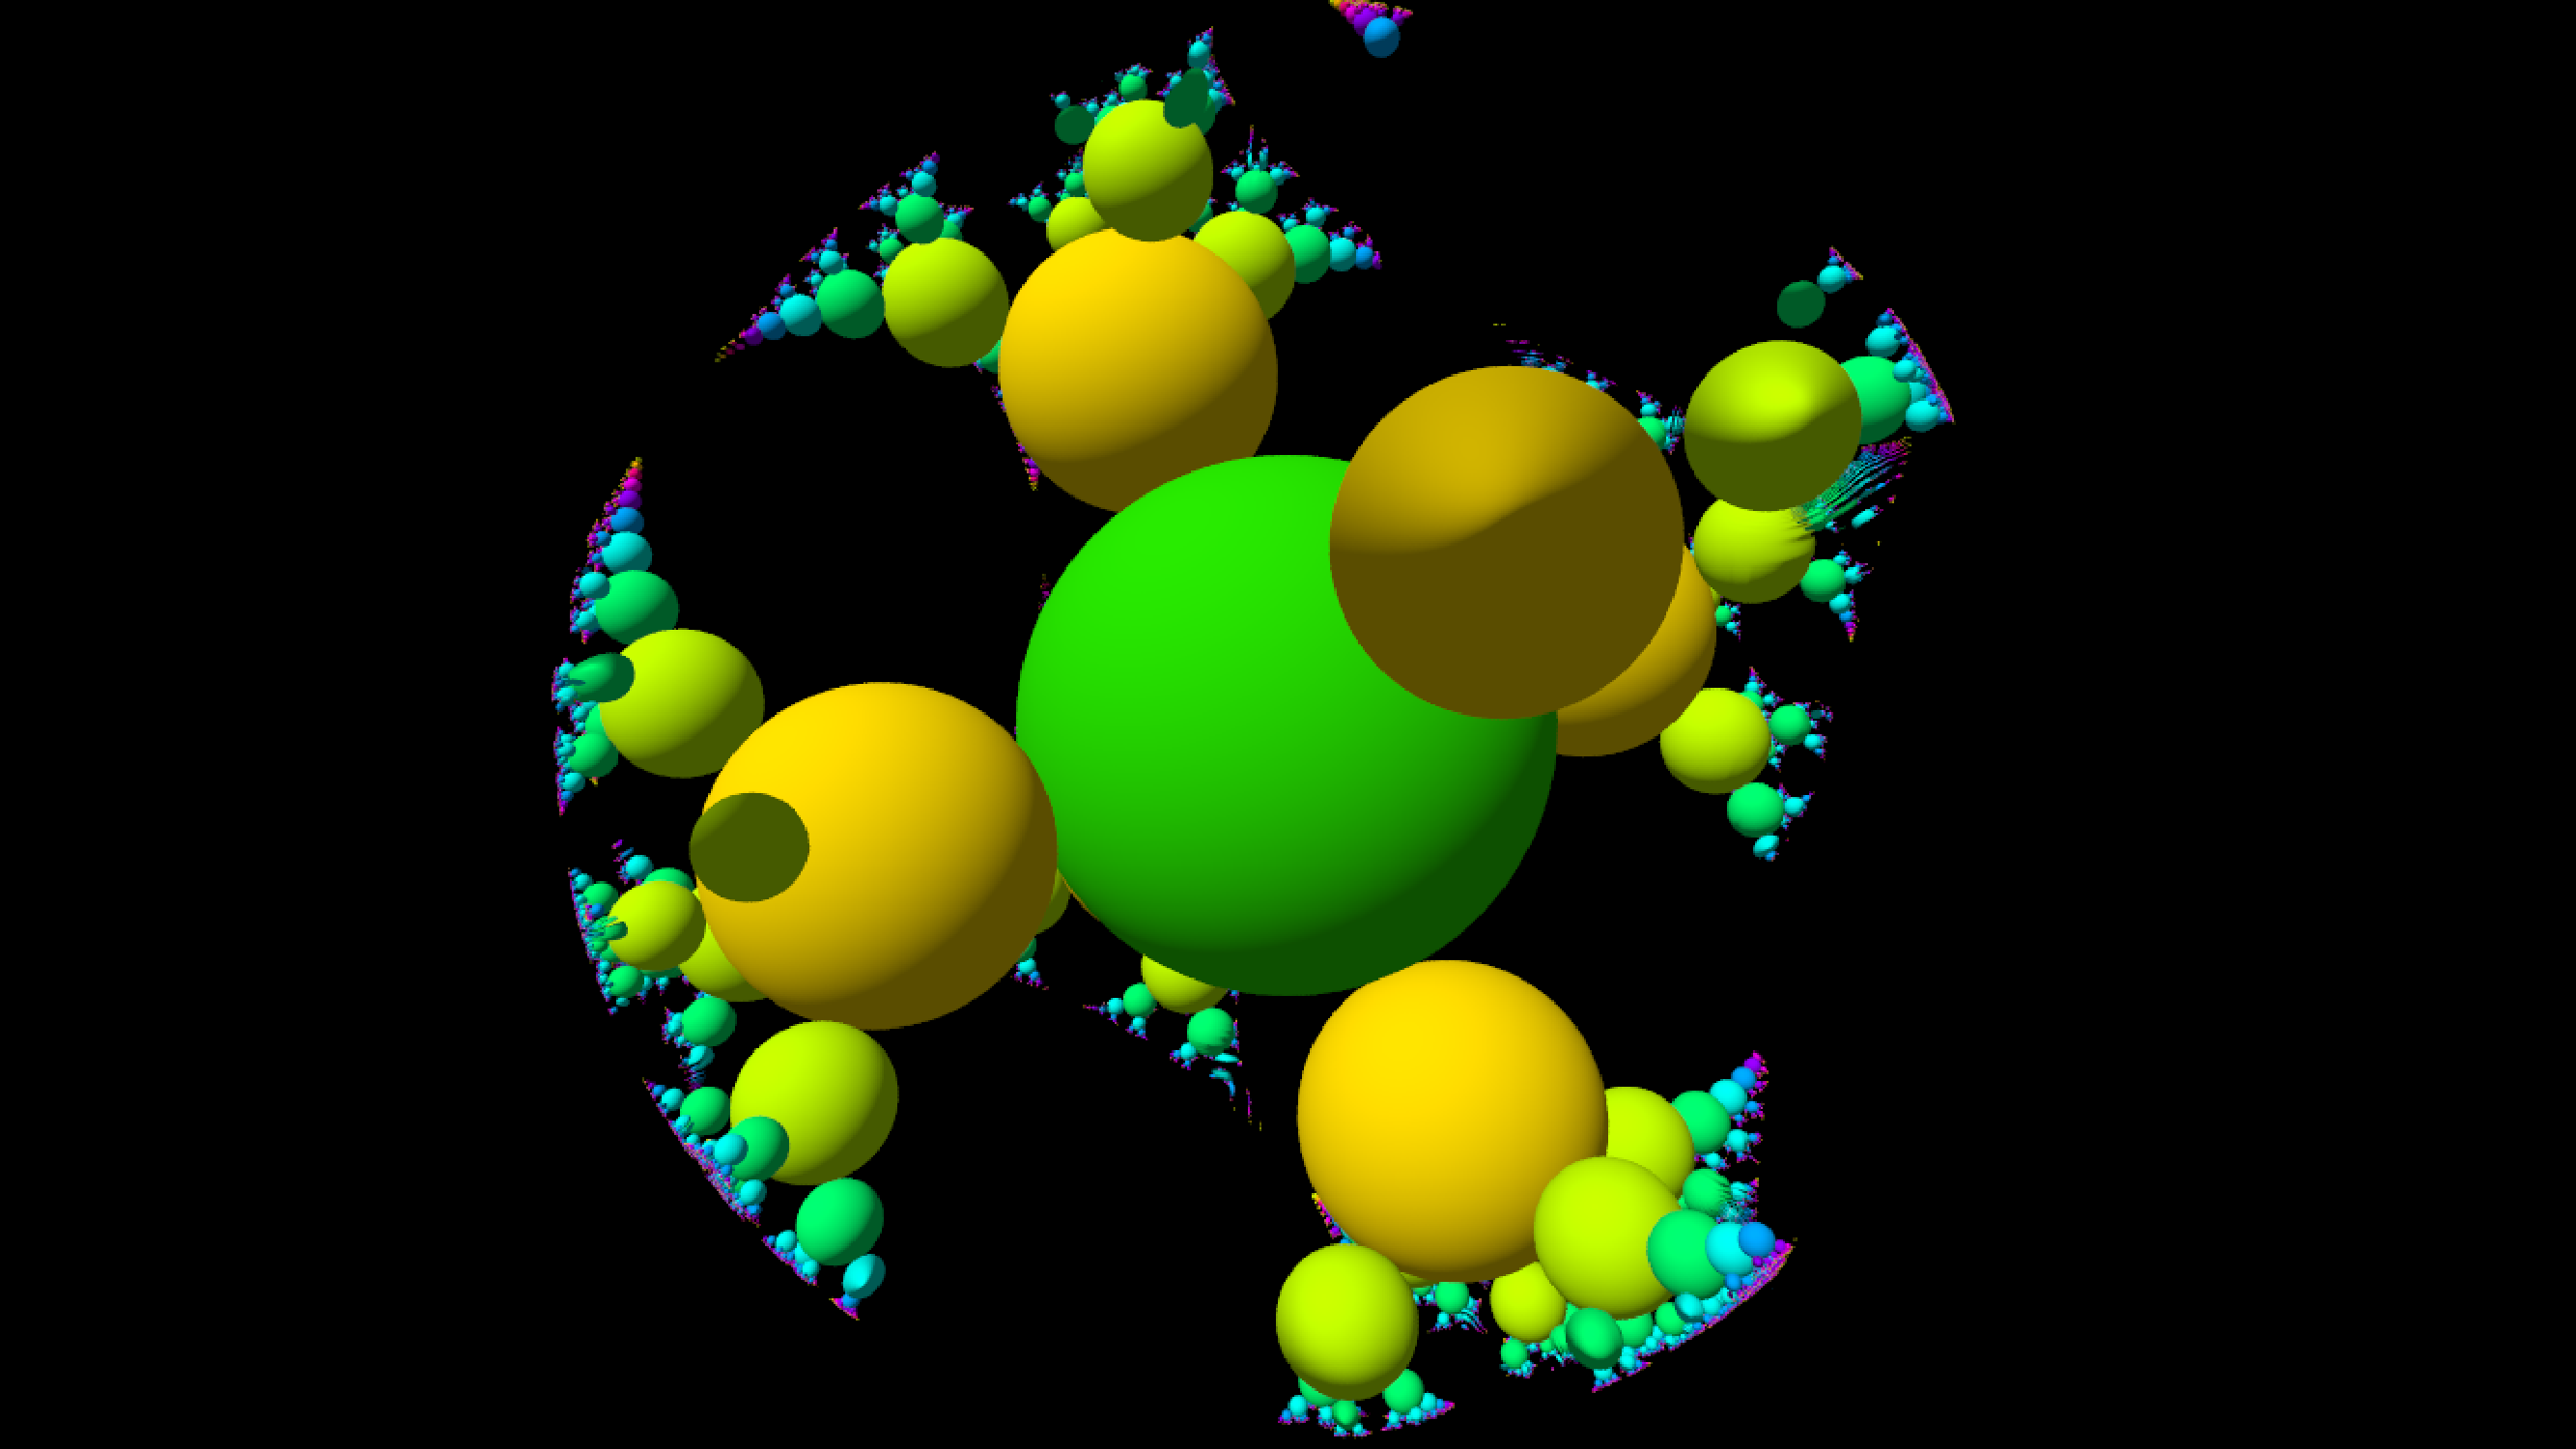
\includegraphics[height=1.35in, keepaspectratio]{img/preparation/artifact.pdf}
  \caption{\textit{artifact}}
  \label{fig:3dartifact}
  \hspace*{\fill}
 \end{minipage}
\end{figure}

In a similar manner to scaling, we can render sphere inversion
fractals.
For the sake of simplicity, we consider a slice image of Figure
\ref{fig:simpleGenOrb}.
See Figure \ref{fig:slice2d}. This image shows the XY-slice of the orbit
of spheres.
Orange disks in the background are slices of the orbit of initial inversion spheres.
Slices of the orbit of the base sphere are colored in
the same color as the orbit shown in Figure \ref{fig:simpleGenOrb}\subref{fig:simpleOrb}.
$C$ is the white circle, the boundary of the initial inversion sphere.
$S1$ is the base sphere and the inversion of $S2$ in the circle $C$. 
The white point $P1$ is the inversion of $P2$ in the circle $C$.

Now we assume that the tip of the ray is at $P2$.
Let's calculate the minimum distance between
$P2$ and the orbit of base spheres.
The nearest sphere to $P2$ is $S2$.
So, we have to calculate the distance between $P2$ and $S2$.
We call the distance $d$.
However, we do not know the center and radius of $S2$.
So, we calculate $d$ from a distance between $S1$ and $P1$.
Inversions in spheres and M\"obius transformations do not preserve
Euclidean distance.
Thus we use the Jacobian to estimate the distance.
We accumulate the Jacobian of inversions by multiplying the Jacobian for
every inversion.

Finally, we divide the distance between the base sphere and the point on
the fundamental domain by the accumulated Jacobian, and we can get the
approximated distance between the tip of the ray and the nearest sphere.
For the above case, we get an inequality $d \geq distance(P1, S1)/Jacobian$.
The formula gives a lower bound for spheres.
For more details on the derivation of this estimation formula, see the
blog post\footnote{Inigo Quilez, distance estimation:
\url{http://www.iquilezles.org/www/articles/distance/distance.htm}}
by Inigo Quilez.

We have one more thing to consider because the above calculation is
a rough estimate.
For example, if a given point is in the outer area of the orbit, the
distance function returns unintentionally large distance, and the ray
can pass through the real objects. This causes artifact shown in Figure
\ref{fig:3dartifact}. The fore part of the fractals is not rendered.
In order to avoid this kind of problems, we shrink the length of
the estimated distance.
It increases the number of steps of sphere tracing, but we can
eventually obtain the intersection of the ray and the spheres.
The scaling factor is determined experimentally according to the size of
the spheres.

\begin{algorithm}
 \caption{Distance Function}
 \label{iis3d}
 \begin{algorithmic}
  \REQUIRE count $= 0$, $d$ = MAX\_DISTANCE, $dr = 1.0$, and coordinates
  $=$ tip of the ray
  \FOR{$i=0$ to MAX\_INVERSION}
  \STATE inFundamentalDomain $\leftarrow$ \TRUE
  \FOR{ each Map $G$ in Maps}
  \IF{$G$ is available to coordinates}
  \STATE $dr \leftarrow dr * $ (Jacobian of $G(\text{coordinates})$)
  \STATE coordinates $\leftarrow$ $G(\text{coordinates})$
  \STATE INCREMENT count
  \STATE inFundamentalDomain $\leftarrow$ \FALSE
  \ENDIF
  \ENDFOR
  \IF {inFundamentalDomain}
  \STATE BREAK for
  \ENDIF
  \ENDFOR
  \FOR{ each BaseSphere $S$ in BaseSpheres}
  \STATE $d \leftarrow$ min($d$, scalingFactor $*$ (distance(coordinates, $S$.center) $-$
  $S$.radius) $/$ (absolute value of $dr$))
  \ENDFOR
  \RETURN $d$
 \end{algorithmic}
\end{algorithm}

The generalized pseudo-code for a distance function is in Algorithm \ref{iis3d}. 

\subsection{Related Works}

Aaron Montag uses texture based approach to visualize a limit set of the
Kleinian groups \cite{Montag2014hyperbolicIFS}.
We prepare initial seed circle in the texture.
Next, we apply generators of the group to each pixel.
If the transformed pixel is on the seed circle or filled pixel, we fill the original pixel.
We continue iterating this process; we obtain an image of the limit set of
the group.
This algorithm needs high-resolution texture, and it is difficult to
extend this algorithm to three-dimension.
%% テクスチャベースの描画方法 テクスチャに種となる円を描く,点ごとに,変
%% 換を作用させ,元のテクスチャの円の上にもどってきたらテクスチャを描く
%% これを続けることで極限集合を描画する

\begin{figure}[htbp]
 \begin{minipage}[t]{0.5\hsize}
  \center
  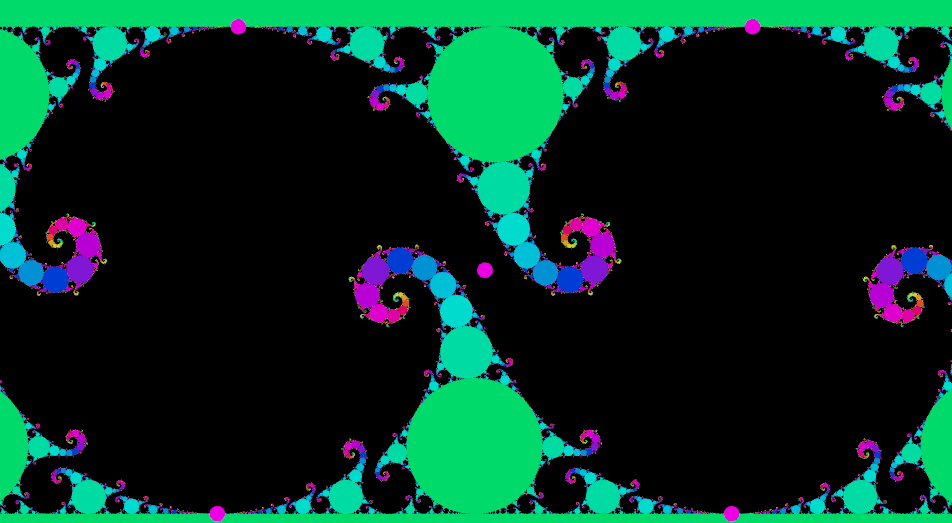
\includegraphics[height=1.35in, keepaspectratio]{img/preparation/related/josklein.png}
  \caption{\textit{}}
  \label{fig:jos}
  \hspace*{\fill}
 \end{minipage}
 \begin{minipage}[t]{0.5\hsize}
  \center
  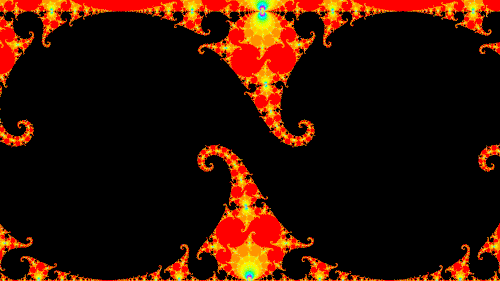
\includegraphics[height=1.35in, keepaspectratio]{img/preparation/related/joskleinInv.png}
  \caption{\textit{}}
  \label{fig:josInv}
  \hspace*{\fill}
 \end{minipage}
\end{figure}

Jos Leys invented efficient algorithm to draw a Kleinian group with Maskit
parametrization shown in Figure
\ref{fig:jos}\footnote{\url{http://www.josleys.com/article_show.php?id=221}}. 
The pink points are control points of the fractal.
IIS uses circle or sphere inversions, on the other hand, Jos Leys used
M\"obius transformations algebraically.
He observes the orbit of the Maskit parametrization group and
successfully discover the algorithm to visualize Maskit groups.
We can apply circle inversions to his figure, and we obtain Figure \ref{fig:josInv}.

Martin von Gagern and J\"urgen Richter-Gebert introduce an algorithm
called \textit{Reverse Pixel Lookup}
\cite{journals/combinatorics/GagernR09} to render two-dimensional
hyperbolic tiling.
The algorithm is similar to ours, but
we explore the method not only tiling but also other varieties of
images, for instance, three-dimensional objects.
